% METODOLOGIA------------------------------------------------------------------

\chapter{METODOLOGIA}
\label{chap:metodologia}


\section{Análise e definição das características do projeto}

Para a metodologia deste trabalho de conclusão de curso, partiu-se do princípio de uma estrutura previamente construída, demostrada no esquema abaixo. A partir dos elementos dessa figura, evidenciados na \autoref{tab:tabela_esquema_cisterna}, foi possível realizar uma análise sobre o que pode ser automatizado, levando em consideração as variáveis e características do sistema.  

\begin{figure}[H]
	\centering
	\caption{Esquema de demonstração de uma cisterna no subsolo}
	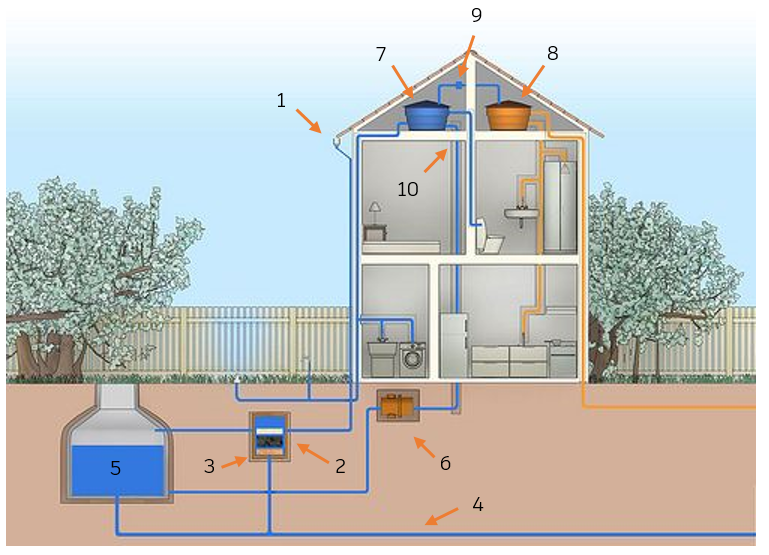
\includegraphics[width=1.0\textwidth]{figuras/esquema_cisterna.png}
	\fonte{Adaptado (ECOMONTES, 2016)}
	\label{fig:esquema_cisterna}
\end{figure}

\newpage

\begin{table}[]
	\centering
	\small
	\begin{tabular}{c|c|c}
		\hline
		\textbf{Identificador} & \textbf{Elemento} & \textbf{Descrição} \\ \hline
		1 & Calha coletora & \begin{tabular}[c]{@{}c@{}}Elemento convencional para coleta e \\ descarte de água da chuva\end{tabular} \\ \hline
		2 & Filtro A (cascalho fino) & \begin{tabular}[c]{@{}c@{}}Elemento para realização de \\ filtragem de pequenas impurezas\end{tabular} \\ \hline
		3 & Filtro B (cascalho grosso) & \begin{tabular}[c]{@{}c@{}}Elemento para realização de \\ filtragem de impurezas\end{tabular} \\ \hline
		4 & Tubulação de descarte & \begin{tabular}[c]{@{}c@{}}Tubulação utilizada como rota de escoamento \\ quando o reservatório não está em uso ou \\ está cheio\end{tabular} \\ \hline
		5 & Reservatório de coleta & Cisterna propriamente dita \\ \hline
		6 & Motobomba ou bomda d'água & \begin{tabular}[c]{@{}c@{}}Elemento utilizado para realização do \\ ganho de elevação da água\end{tabular} \\ \hline
		7 & Caixa d'água auxiliar & \begin{tabular}[c]{@{}c@{}}Caixa d'água convencional com alimentação \\ oriunda da bomba d'água\end{tabular} \\ \hline
		8 & Caixa d'água convencional & \begin{tabular}[c]{@{}c@{}}Caixa d'água padrão com alimentação \\ da estação de água da cidade\end{tabular} \\ \hline
		9 & Elo de ligação & \begin{tabular}[c]{@{}c@{}}Ligação utilizada para abastecer a caixa d'água \\ auxiliar quando a cisterna está seca \\ ou em manutenção\end{tabular} \\ \hline
		10 & Distribuidor & \begin{tabular}[c]{@{}c@{}}Elementos de distribuição de água \\ para pontos estratégicos\end{tabular} \\ \hline
	\end{tabular}
	\caption{Identificação dos elementos da \autoref{fig:esquema_cisterna}.}
	\label{tab:tabela_esquema_cisterna}
\end{table}
% https://www.tablesgenerator.com

Com base nesses elementos é importante destacar os seguintes pontos para as implementações que serão tratadas nas seções posteriores:

\begin{itemize}
	\item Definir o método ou sistema para medição de nível do item 5;
	\item Elaborar o sistema de ativação/desativação da motobomba do item 6;
	\item Definir o método ou sistema para medição de nível do item 7;
	\item Elaborar um sistema para intermediar/controlar a passagem de água no elo de ligação (item 9);
	\item Definir um sistema para administrar o descarte de água da cisterna (item 4);
	\item Esquematizar e situar os sistemas para envio e aquisição de dados, tornando-se possível realizar remotamente as operações citadas nos itens anteriores; 
	\item Configurar um pequeno servidor para intermediar entre os dispositivos microcontrolados e as interfaces de controle;  
	\item Implementar as interfaces para visualizar/comandar os pontos citados nos itens anteriores.
\end{itemize}

Dois módulos distintos foram propostos: \textbf{\textit{Tank Control Module} - TCM}, o qual será responsável pelo monitoramento e controle da caixa d'água auxiliar (\autoref{fig:esquema_cisterna}, identificador 7) e \textbf{\textit{Cistern Control Module} - CCM}, responsável pelo monitoramento e controle da cisterna (\autoref{fig:esquema_cisterna}, identificador 5). O diagrama da \autoref{fig:esquema_proj} mostra o esquema proposto para a criação do projeto. 

\begin{figure}[H]
	\centering
	\caption{Esquema básico do projeto.}
	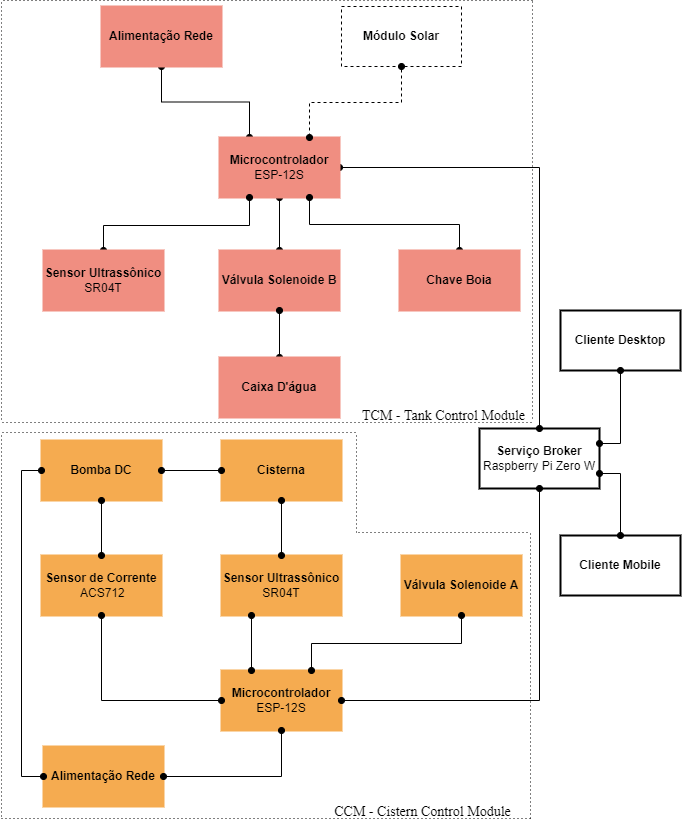
\includegraphics[width=1\textwidth]{figuras/esquema_basico_proj_2.png}
	\fonte{Própria}
	\label{fig:esquema_proj}
\end{figure}

Outro ponto importante desta parte do projeto foi estabelecer as medidas de volume da cisterna e da caixa d'água assim como as equações de volume tendo como variável a altura do líquido. Para a cisterna, considerou-se um reservatório no formado de um paralelepípedo retângulo, com as dimensões definidas:

\begin{figure}[H]
	\centering
	\caption{Representação das dimensões da cisterna.}
	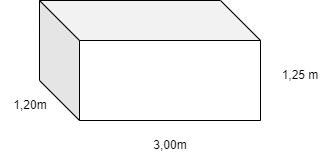
\includegraphics[width=0.4\textwidth]{figuras/volume.png}
	\fonte{Própria}
	\label{fig:volume_cisterna}
\end{figure}

Equação de volume associada:

\begin{equation}
V = c \cdot l \cdot (h-s)  
\end{equation}

\begin{itemize}
	\item $V$ é o volume;
	\item $h$ é a altura do tanque;
	\item $s$ é a leitura de distância do sensor;
	\item $c$ é o comprimento do tanque;
	\item $l$ é o largura do tanque. \\
\end{itemize}

Para a caixa d'água, considerou-se um reservatório de 1000L, no formato de tronco de cone (formato padrão):

\begin{figure}[H]
	\centering
	\caption{Representação das dimensões da caixa d'água (valores em centímetros).}
	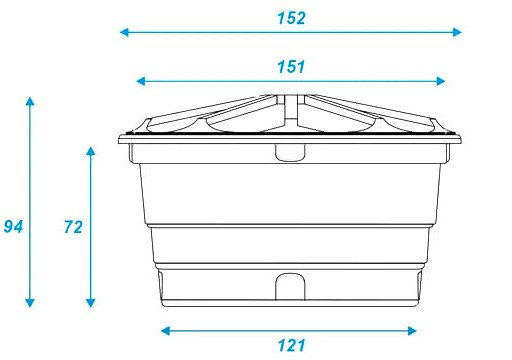
\includegraphics[width=0.5\textwidth]{figuras/caixa.jpg}
	\fonte{tendtudo.com, 2021}
	\label{fig:volume_tanque}
\end{figure}

Equação de volume associada:

\begin{equation}
V = \frac{\pi\cdot (h-s)\cdot (R^{2}+R\cdot r+r^{2})}{3} 
\end{equation}

\begin{itemize}
	\item $V$ é o volume;
	\item $h$ é a altura do tanque;
	\item $s$ é a leitura de distância do sensor;
	\item $R$ é o raio maior;
	\item $r$ é o raio menor.
\end{itemize}




\section{Organização do trabalho}

Iniciou-se com a criação do quadro \textit{Kanban} (\autoref{fig:kanban-proj}), para auxílio da organização das tarefas, e com a criação do repositório no \textit{Github} (\autoref{fig:github}) para armazenamento e versionamento dos códigos das vertentes de \textit{Firmware} e \textit{Software} do projeto. Deu-se prosseguimento com os estudos e levantamentos bibliográficos relacionando três áreas do projeto. Buscou-se encontrar os métodos,  ferramentas, tecnologias, bibliotecas e \textit{frameworks} mais adequados para a implementação do projeto.  Diante de cada seleção feita, foram executadas análises para que fosse definido o funcionamento do sistema total, munido da combinação de cada uma das três áreas citadas anteriormente e visando a geração de um produto que pudesse ser empregado no mercado: atrativo economicamente e seguindo diretrizes sustentáveis.  

Primeiramente, na seção de \textit{hardware}, foram selecionados as ferramentas criação e simulação de circuitos, a escolha de todos os dispositivos eletrônicos a serem utilizados e a análise do local de aplicação. Posteriormente, na parte de \textit{firmware}, já estando selecionados os microcontroladores e o microprocessador, foram determinadas todas as rotinas de operação e escolhidas, respectivamente, as linguagens para programá-los e o sistema operacional a ser utilizado no microprocessador. Na parte de \textit{software}, foram selecionadas as ferramentas para a criação de interfaces dentro da camada \textit{front-end}: aplicações \textit{mobile} e \textit{desktop}.

Por fim, elaborou-se a lista de materiais necessários para construção o projeto, tendo objetivo de validação em ambiente real, efetuando testes de longos períodos, averiguando a integridade do sistema, a robustez dos componentes e a identificação de casos não previstos anteriormente, tornando possível a aplicação de melhorias posteriores a entrega deste trabalho.

\begin{figure}[H]
	\centering
	\caption{Visão geral do quadro \textit{Kanban} criado na ferramenta \textit{Trello}}
	\includegraphics[width=0.85\textwidth]{figuras/visão_geral_meu_kanban.png}
	\fonte{Própria.}
	\label{fig:kanban-proj}
\end{figure}


\begin{figure}[H]
	\centering
	\caption{Visão geral repositório criado no \textit{Github}}
	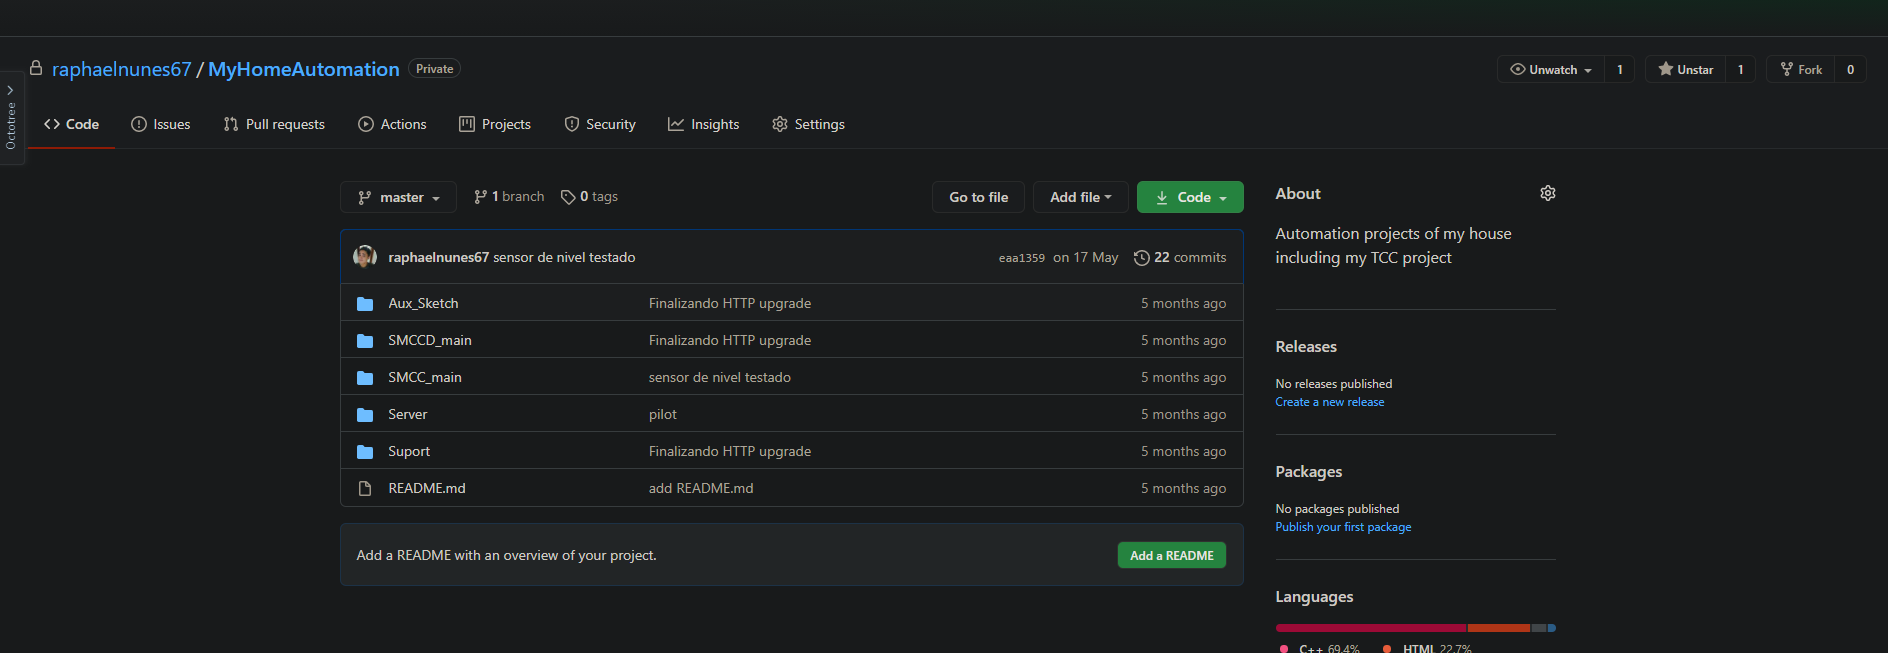
\includegraphics[width=0.85\textwidth]{figuras/github.png}
	\fonte{Própria.}
	\label{fig:github}
\end{figure}



\section{Levantamento do referencial bibliográfico e capacitação}
\label{sec:metmodal}

Essa parte do trabalho conteve-se no levantamento de referências bibliográficas relacionadas com os temas de \textit{IoT}, programação de microcontroladores, criação de aplicações com \textit{frameworks} baseados em \textit{Javascript}. Também buscou-se a capacitação em cursos oferecidos pelas plataformas \textit{Alura}, \textit{Udemy} e \textit{Skylab (Rocketseat)} o aprendizado de conteúdos complementares ao curso de formação em engenheria de controle e automação, como a criação de placas de circuito impresso, treinamentos sobre \textit{Linux} embarcado, implementação do protocolo \textit{MQTT}, criação de \textit{APPs Android} com \textit{React Native} e aplicações \textit{Desktop} com \textit{Electron.js}.

\section{Desenvolvimento dos elementos de \textit{Hardware}}
\label{sec: dev_ele_hw}

Nesse momento foram definidos todos os elementos de \textit{hardware} necessários para o desenvolvimento do trabalho: dispositivos eletrônicos, documentos como \textit{Datasheets}, catálogos e informativos de dispositivos elétricos. Realizou-se uma busca no mercado pelos componentes necessários, posteriormente, efetuando compras para a execução de testes.

\subsection{O circuito de alimentação}

Nesta etapa do projeto iniciou-se a criação do circuito de alimentação para os módulos \textbf{CCM} e \textbf{TCM}. Partindo-se da fonte chaveada definida no \autoref{chap:fundamentacao-teorica}, a qual transforma 110V AC em 12V DC, criou-se um conversor DC-DC do tipo \textit{Buck} para converter a tensão de saída da fonte para 3.3V, ideais para alimentação dos sensores e microcontroladores. 

\begin{figure}[H]
	\centering
	\caption{Esquma de ligação do circuito de alimentação}
	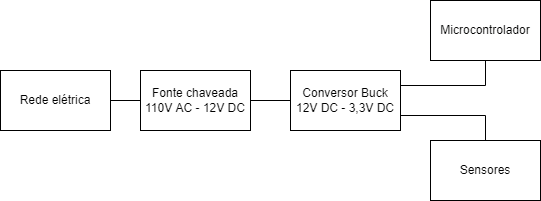
\includegraphics[width=0.8\textwidth]{figuras/alimentacao.png}
	\fonte{Própria.}
	\label{fig:alimentacao_esquema}
\end{figure}

Após a definição do esquema de medição, procurou-se dimensionar o conversor \textit{Buck}. O dimensionamento deu-se a partir das leituras dos \textit{datasheets} de todos os dispositivos que futuramente poderiam ser utilizados. Outro ponto importante salientar para a escolha do conversor \textit{Buck} foi a disponibilidade no mercado.

Dentre os fatores citados o conversor selecionado foi o LM2596, o qual podemos encontrar um módulo com sua aplicação típica (\autoref{fig:conversor_buck}) com certa facilidade no mercado. A \autoref{fig:conversor_buck_teste} mostra o teste realizado em bancada.

\begin{figure}[H]
	\centering
	\caption{Aplicação típica do LM2596.}
	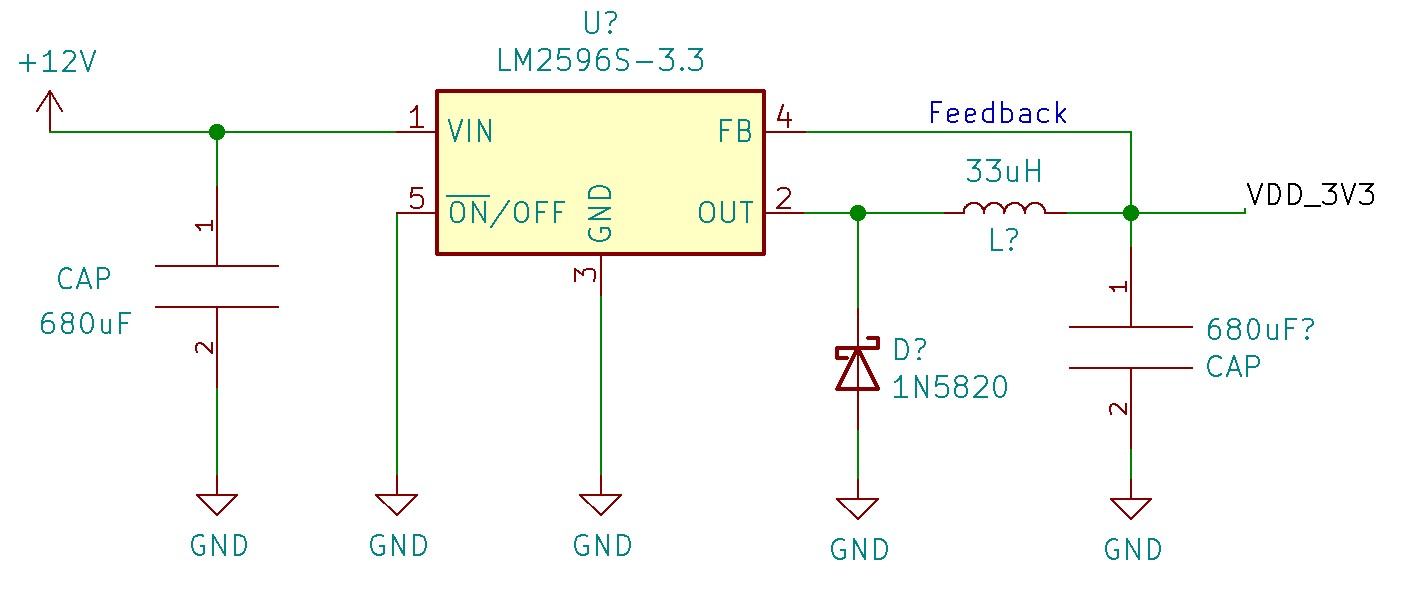
\includegraphics[width=0.8\textwidth]{figuras/conversor_buck.jpg}
	\fonte{Própria.}
	\label{fig:conversor_buck}
\end{figure}

\begin{figure}[H]
	\centering
	\caption{Teste em bancada do módulo com LM2596.}
	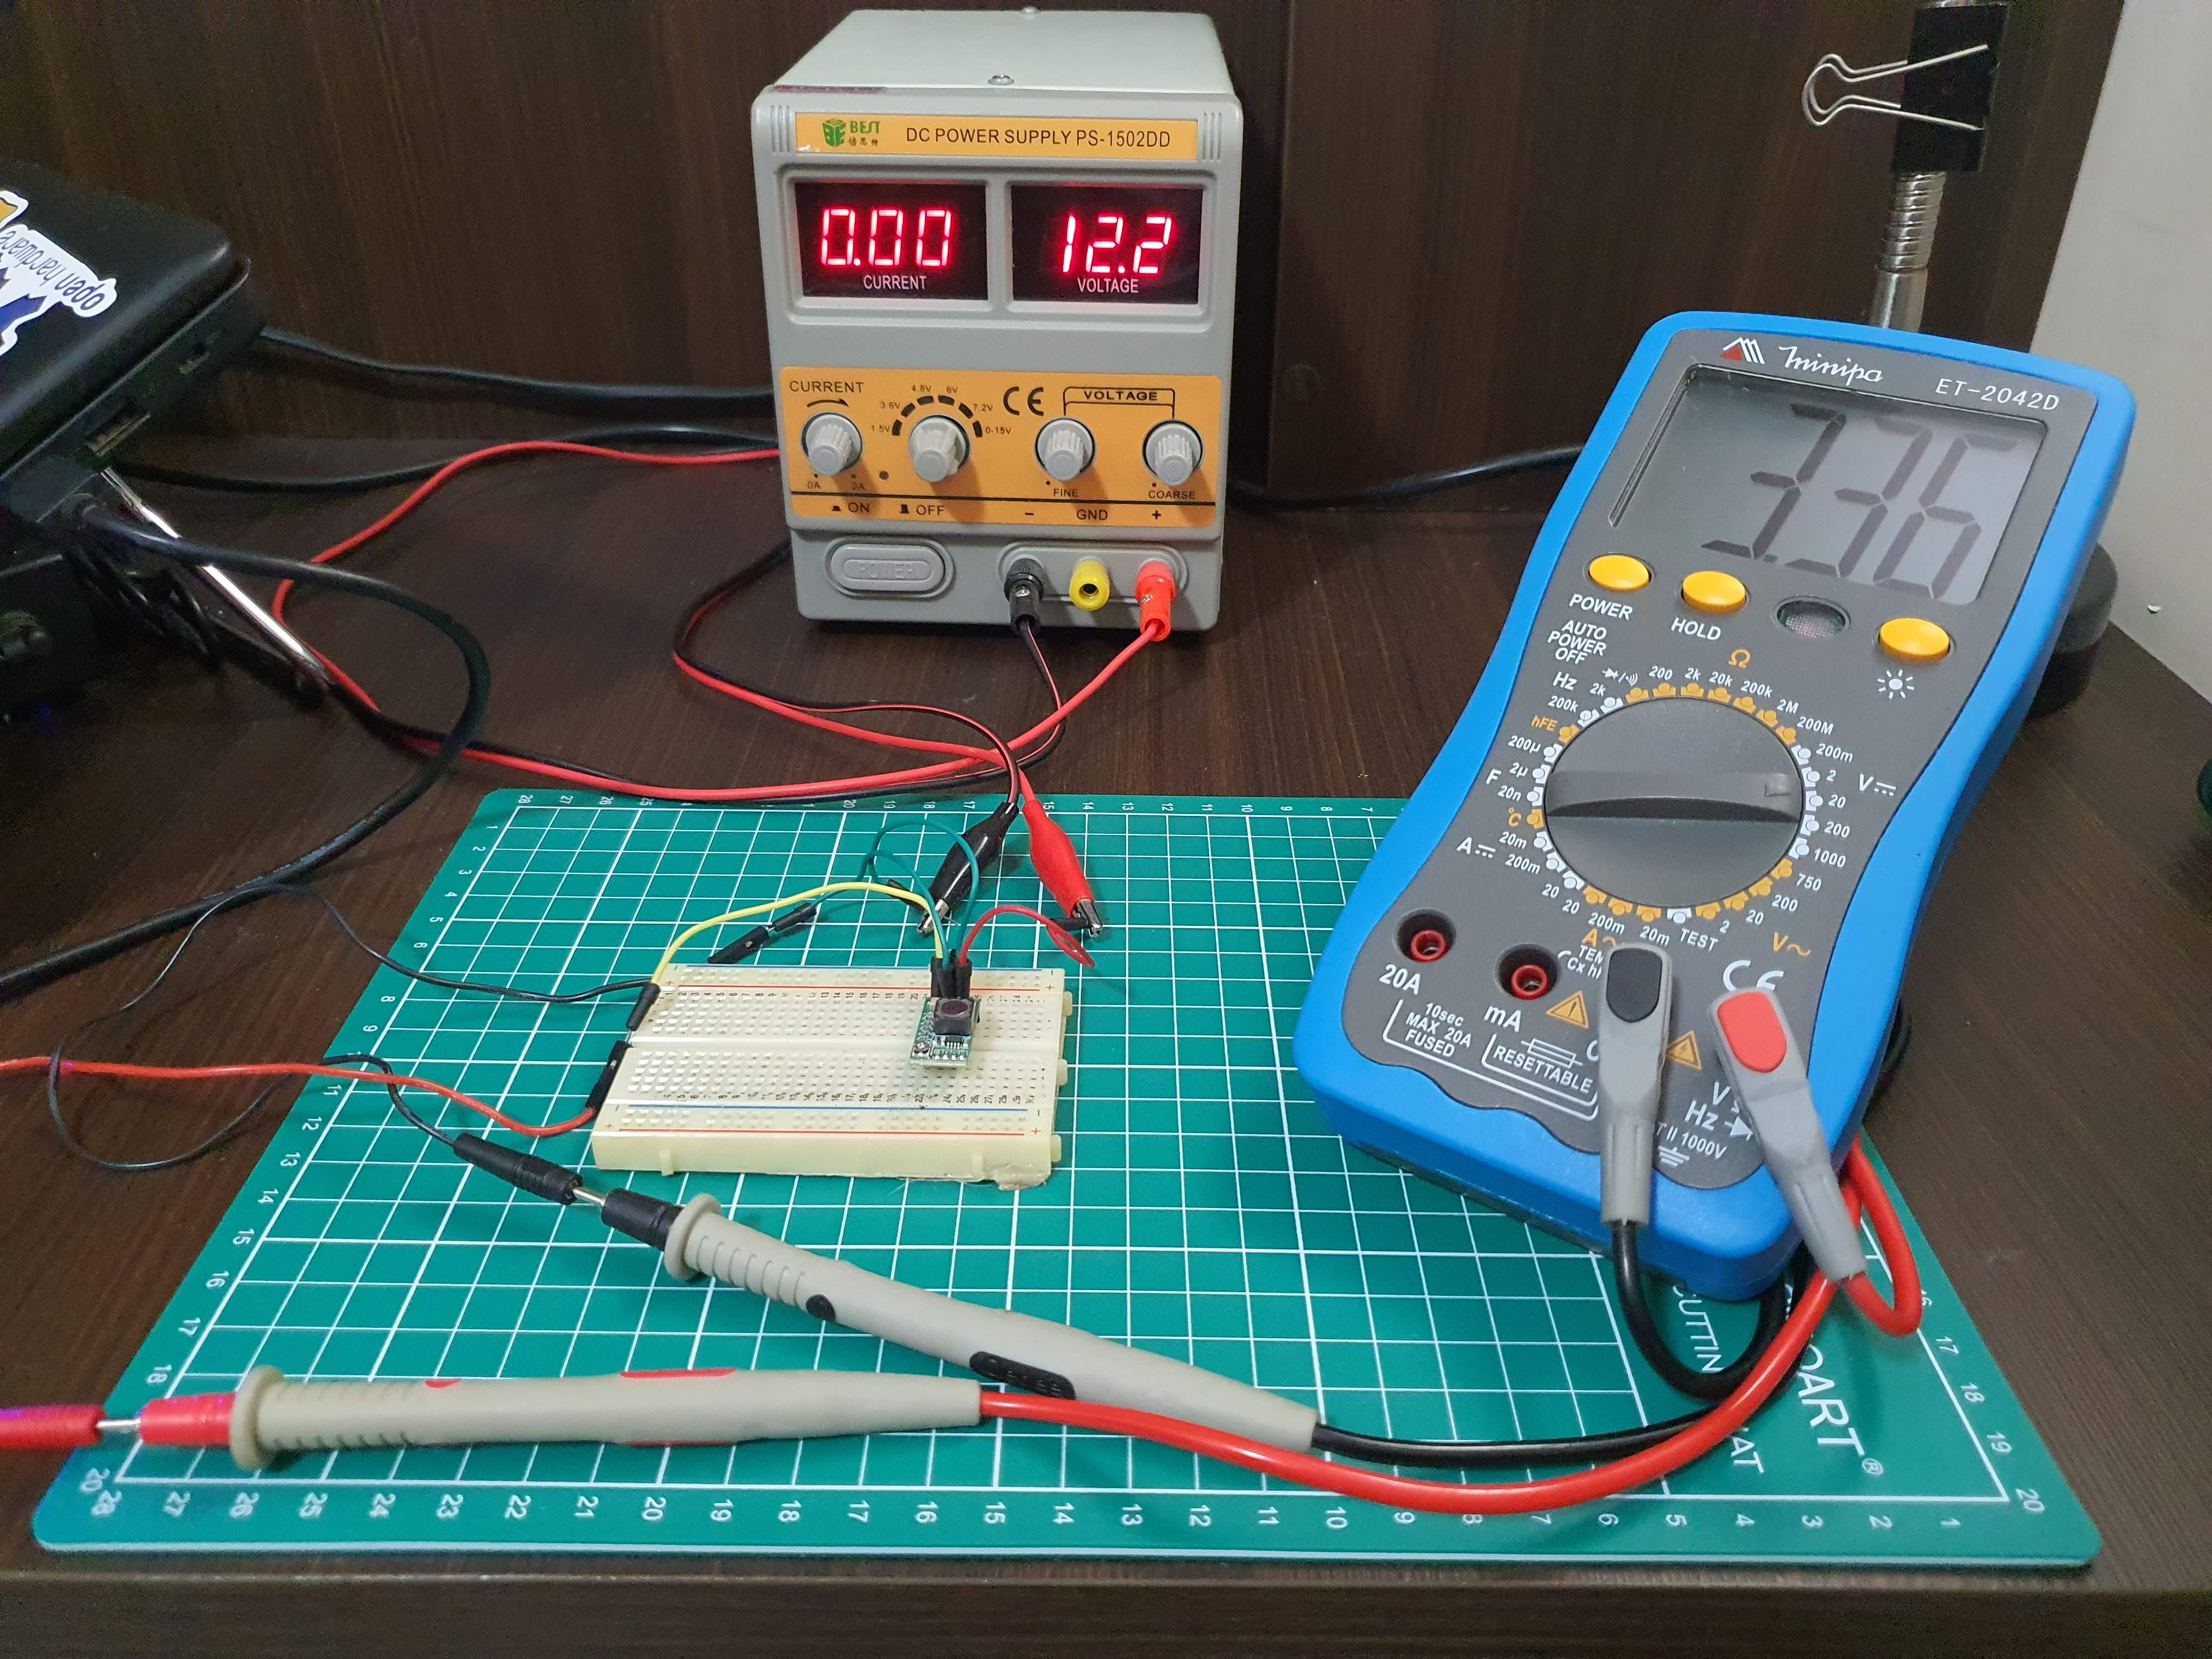
\includegraphics[width=0.7\textwidth]{figuras/conversor_buck_teste.jpg}
	\fonte{Própria.}
	\label{fig:conversor_buck_teste}
\end{figure}

\subsection{O circuito de detecção de fechadura da chave}

 Garantindo a redundância do sistema, no quesito de segurança, planejou-se a aplicação de uma chave tipo boia para ser acoplada a caixa d'água do módulo TCM (\autoref{fig:chave_boia_aplicacao}). Essa chave tem como objetivo garantir que não ocorra vazamento durante o processo de enchimento do tanque.

\begin{figure}[H]
	\centering
	\caption{Esquema de aplicação da chave boia}
	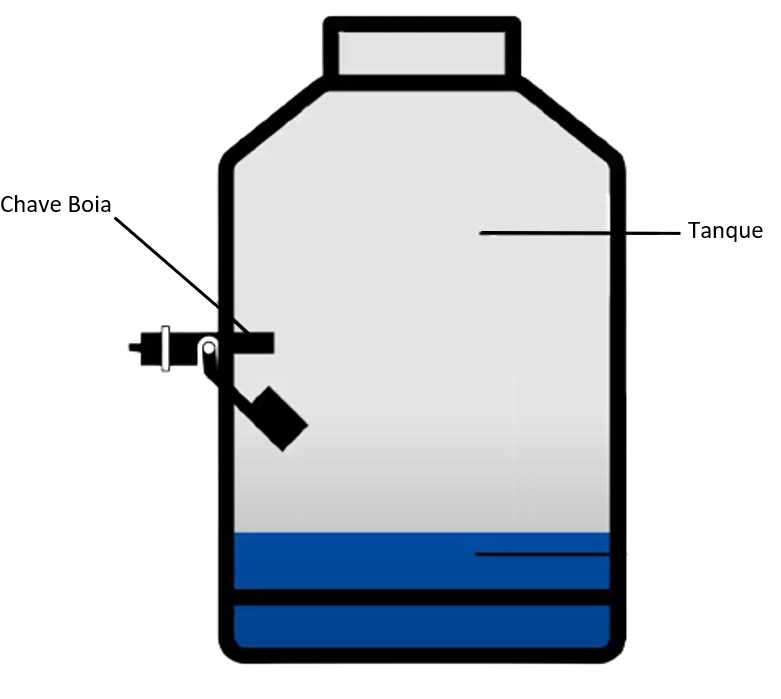
\includegraphics[width=0.4\textwidth]{figuras/chave_boia_aplicacao.png}
	\fonte{Própria.}
	\label{fig:chave_boia_aplicacao}
\end{figure}

Para executar a detecção com essa chave de dois estados foi-se necessário aplicar um circuito com resistores de \textit{pullup} (\autoref{fig:chave_boia_pullup}).

\begin{figure}[H]
	\centering
	\caption{Esquema de ligação elétrica da chave boia.}
	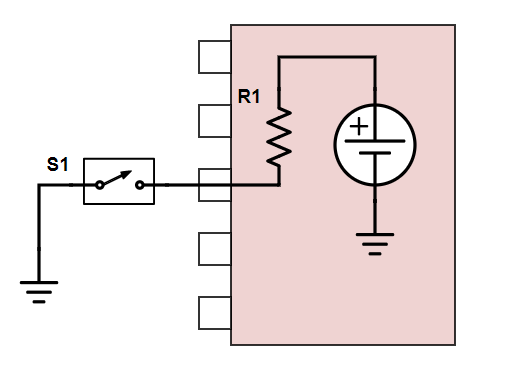
\includegraphics[width=0.4\textwidth]{figuras/pullup.png}
	\fonte{Própria.}
	\label{fig:chave_boia_pullup}
\end{figure}

 Ao definir um pino do microcontrolador como do tipo entrada (\textit{INPUT}), e se em certo momento não houver nada conectado à esse pino, é impossível determinar qual o nível lógico será lido. O esquema de pullup tem o intuito de eliminar tal risco garantindo que apenas dois valores bem definidos sejam lidos no terminal: \textit{HIGH} ou \textit{LOW}.
 
 Em alguns microcontroladores, como no ESP8266, existem alguns pinos que podem se programados como do tipo \textit{pullup}, garantindo que não seja necessário montar um circuito externo para isso. A \autoref{fig:chave_boia_pullup_teste} mostra a montagem realizada em bancada para o teste da chave boia, conectada ao pino digital 5. 
 
 \begin{figure}[H]
 	\centering
 	\caption{Chave boia acoplada ao ESP-12S através de um pino digital com \textit{INPUT PULLUP}.}
 	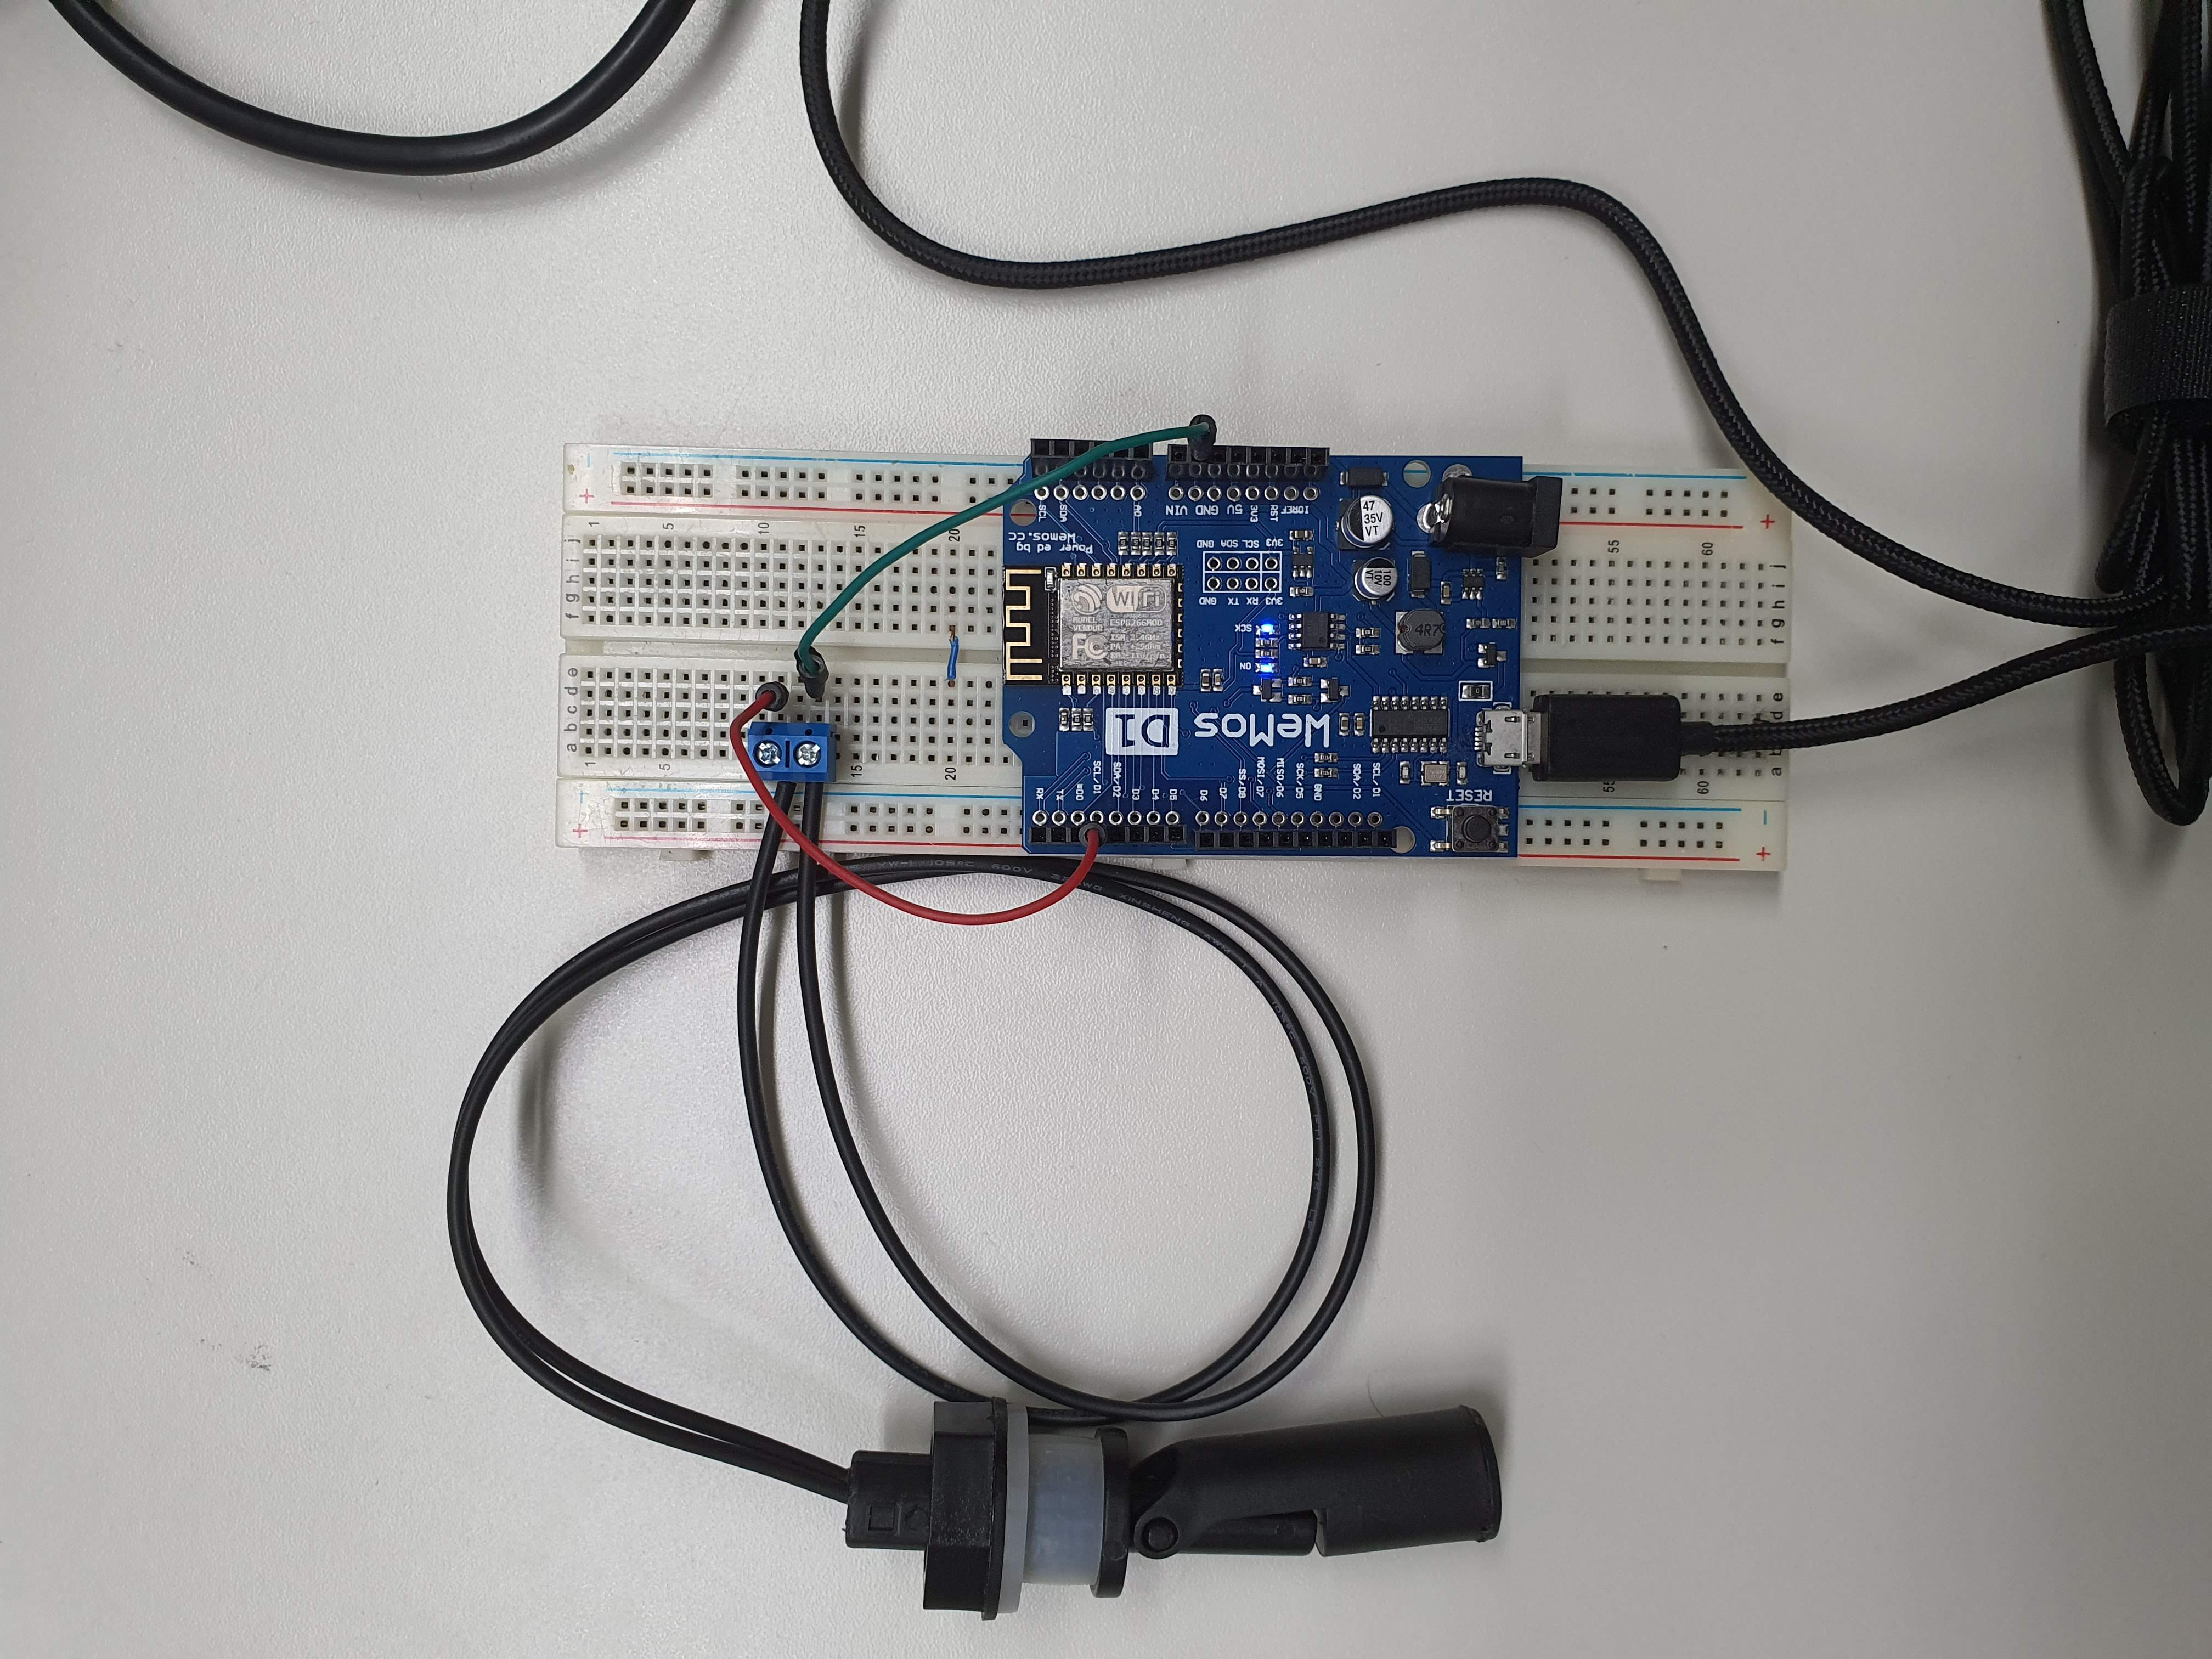
\includegraphics[width=0.6\textwidth]{figuras/teste_chave_boia.jpg}
 	\fonte{Própria.}
 	\label{fig:chave_boia_pullup_teste}
 \end{figure}
 



\subsection{O circuito de medição de nível}

Tendo como base o módulo JSN-SR04T, realizou-se os testes para o envio e recebimento de dados (\autoref{fig:sensor_ultrassonico}). Como descrito na fundamentação teórica, esse módulo possui três tipos de operação, que são selecionadas a partir de um resistor soldado à placa (R27). O modo de operação escolhido para esse projeto foi o terceiro, logo um potenciômetro de $120k\Omega$ (ajustado em $47k\Omega$.) foi soldado à placa (\autoref{fig:ultrasonico_res}). Esse sensor deve estar acoplado, para executar uma leitura precisa, na parte superior do tanque com o seu transceptor apontando diretamente para o líquido. 

 \begin{figure}[H]
	\centering
	\caption{Teste de ligação sensor do módulo JSN-SR04T.}
	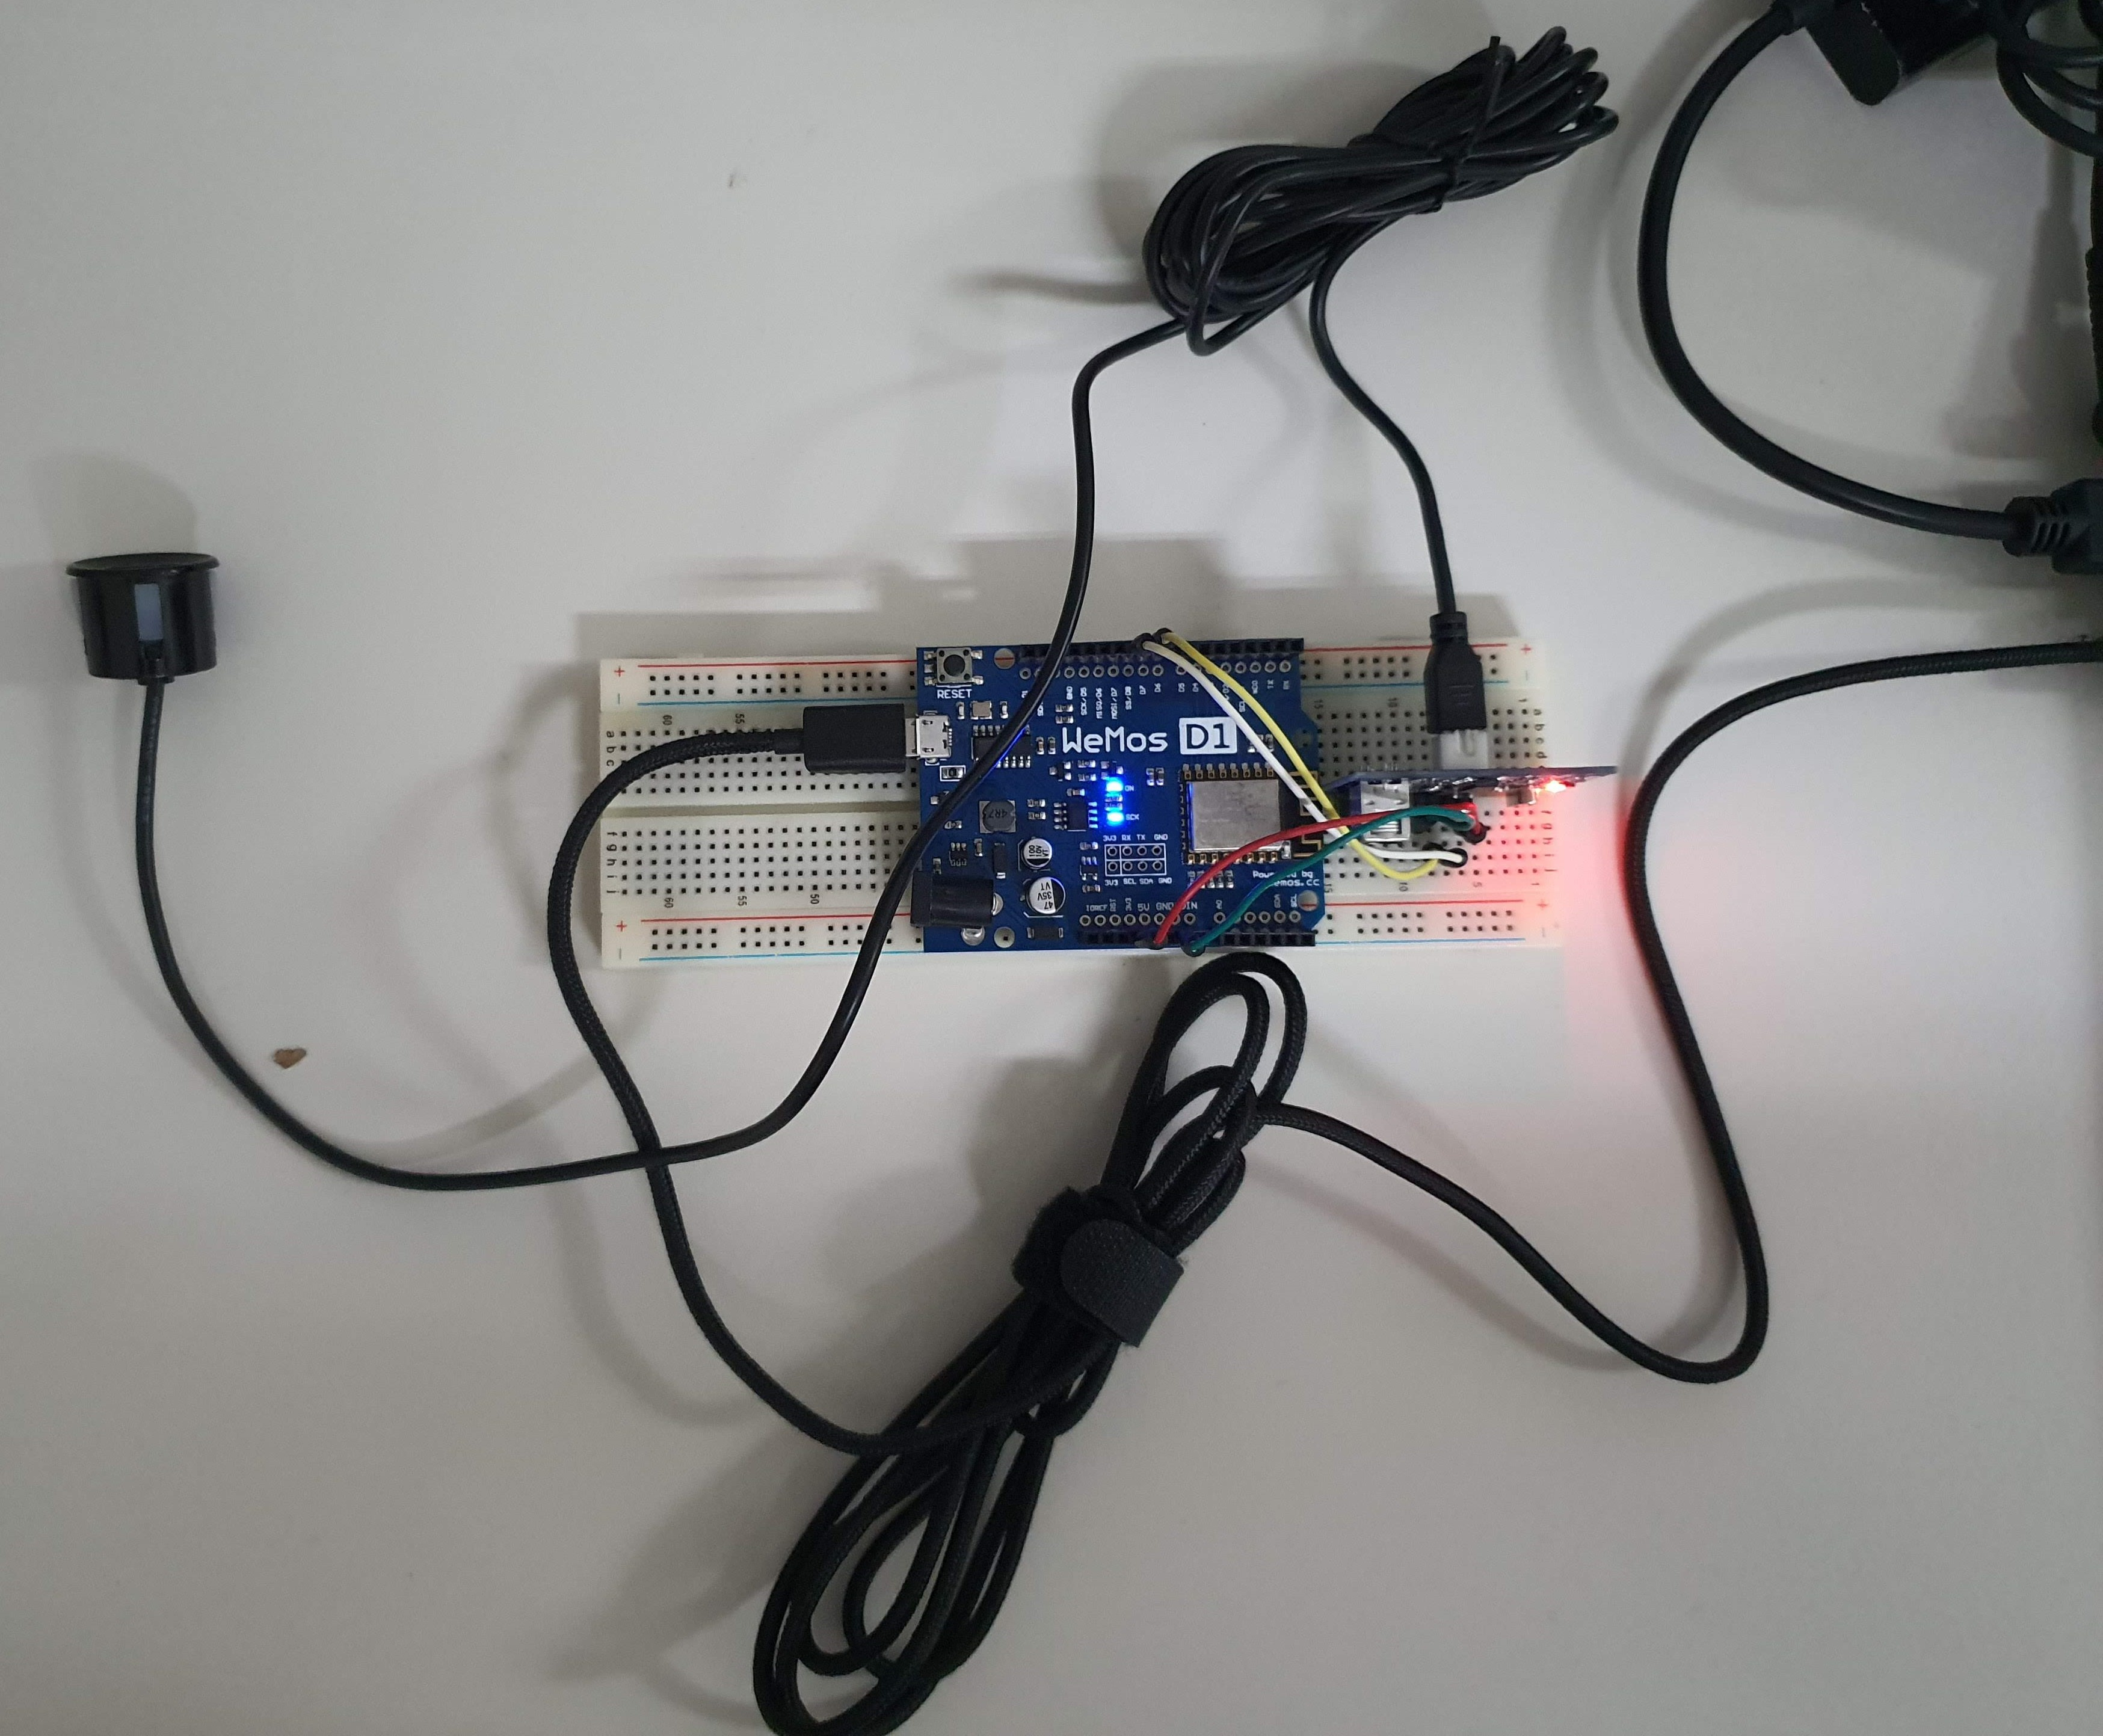
\includegraphics[width=0.6\textwidth]{figuras/teste_ultrassonico.jpg}
	\fonte{Própria.}
	\label{fig:sensor_ultrassonico}
\end{figure}

 \begin{figure}[H]
	\centering
	\caption{Potenciômetro soldado ao módulo.}
	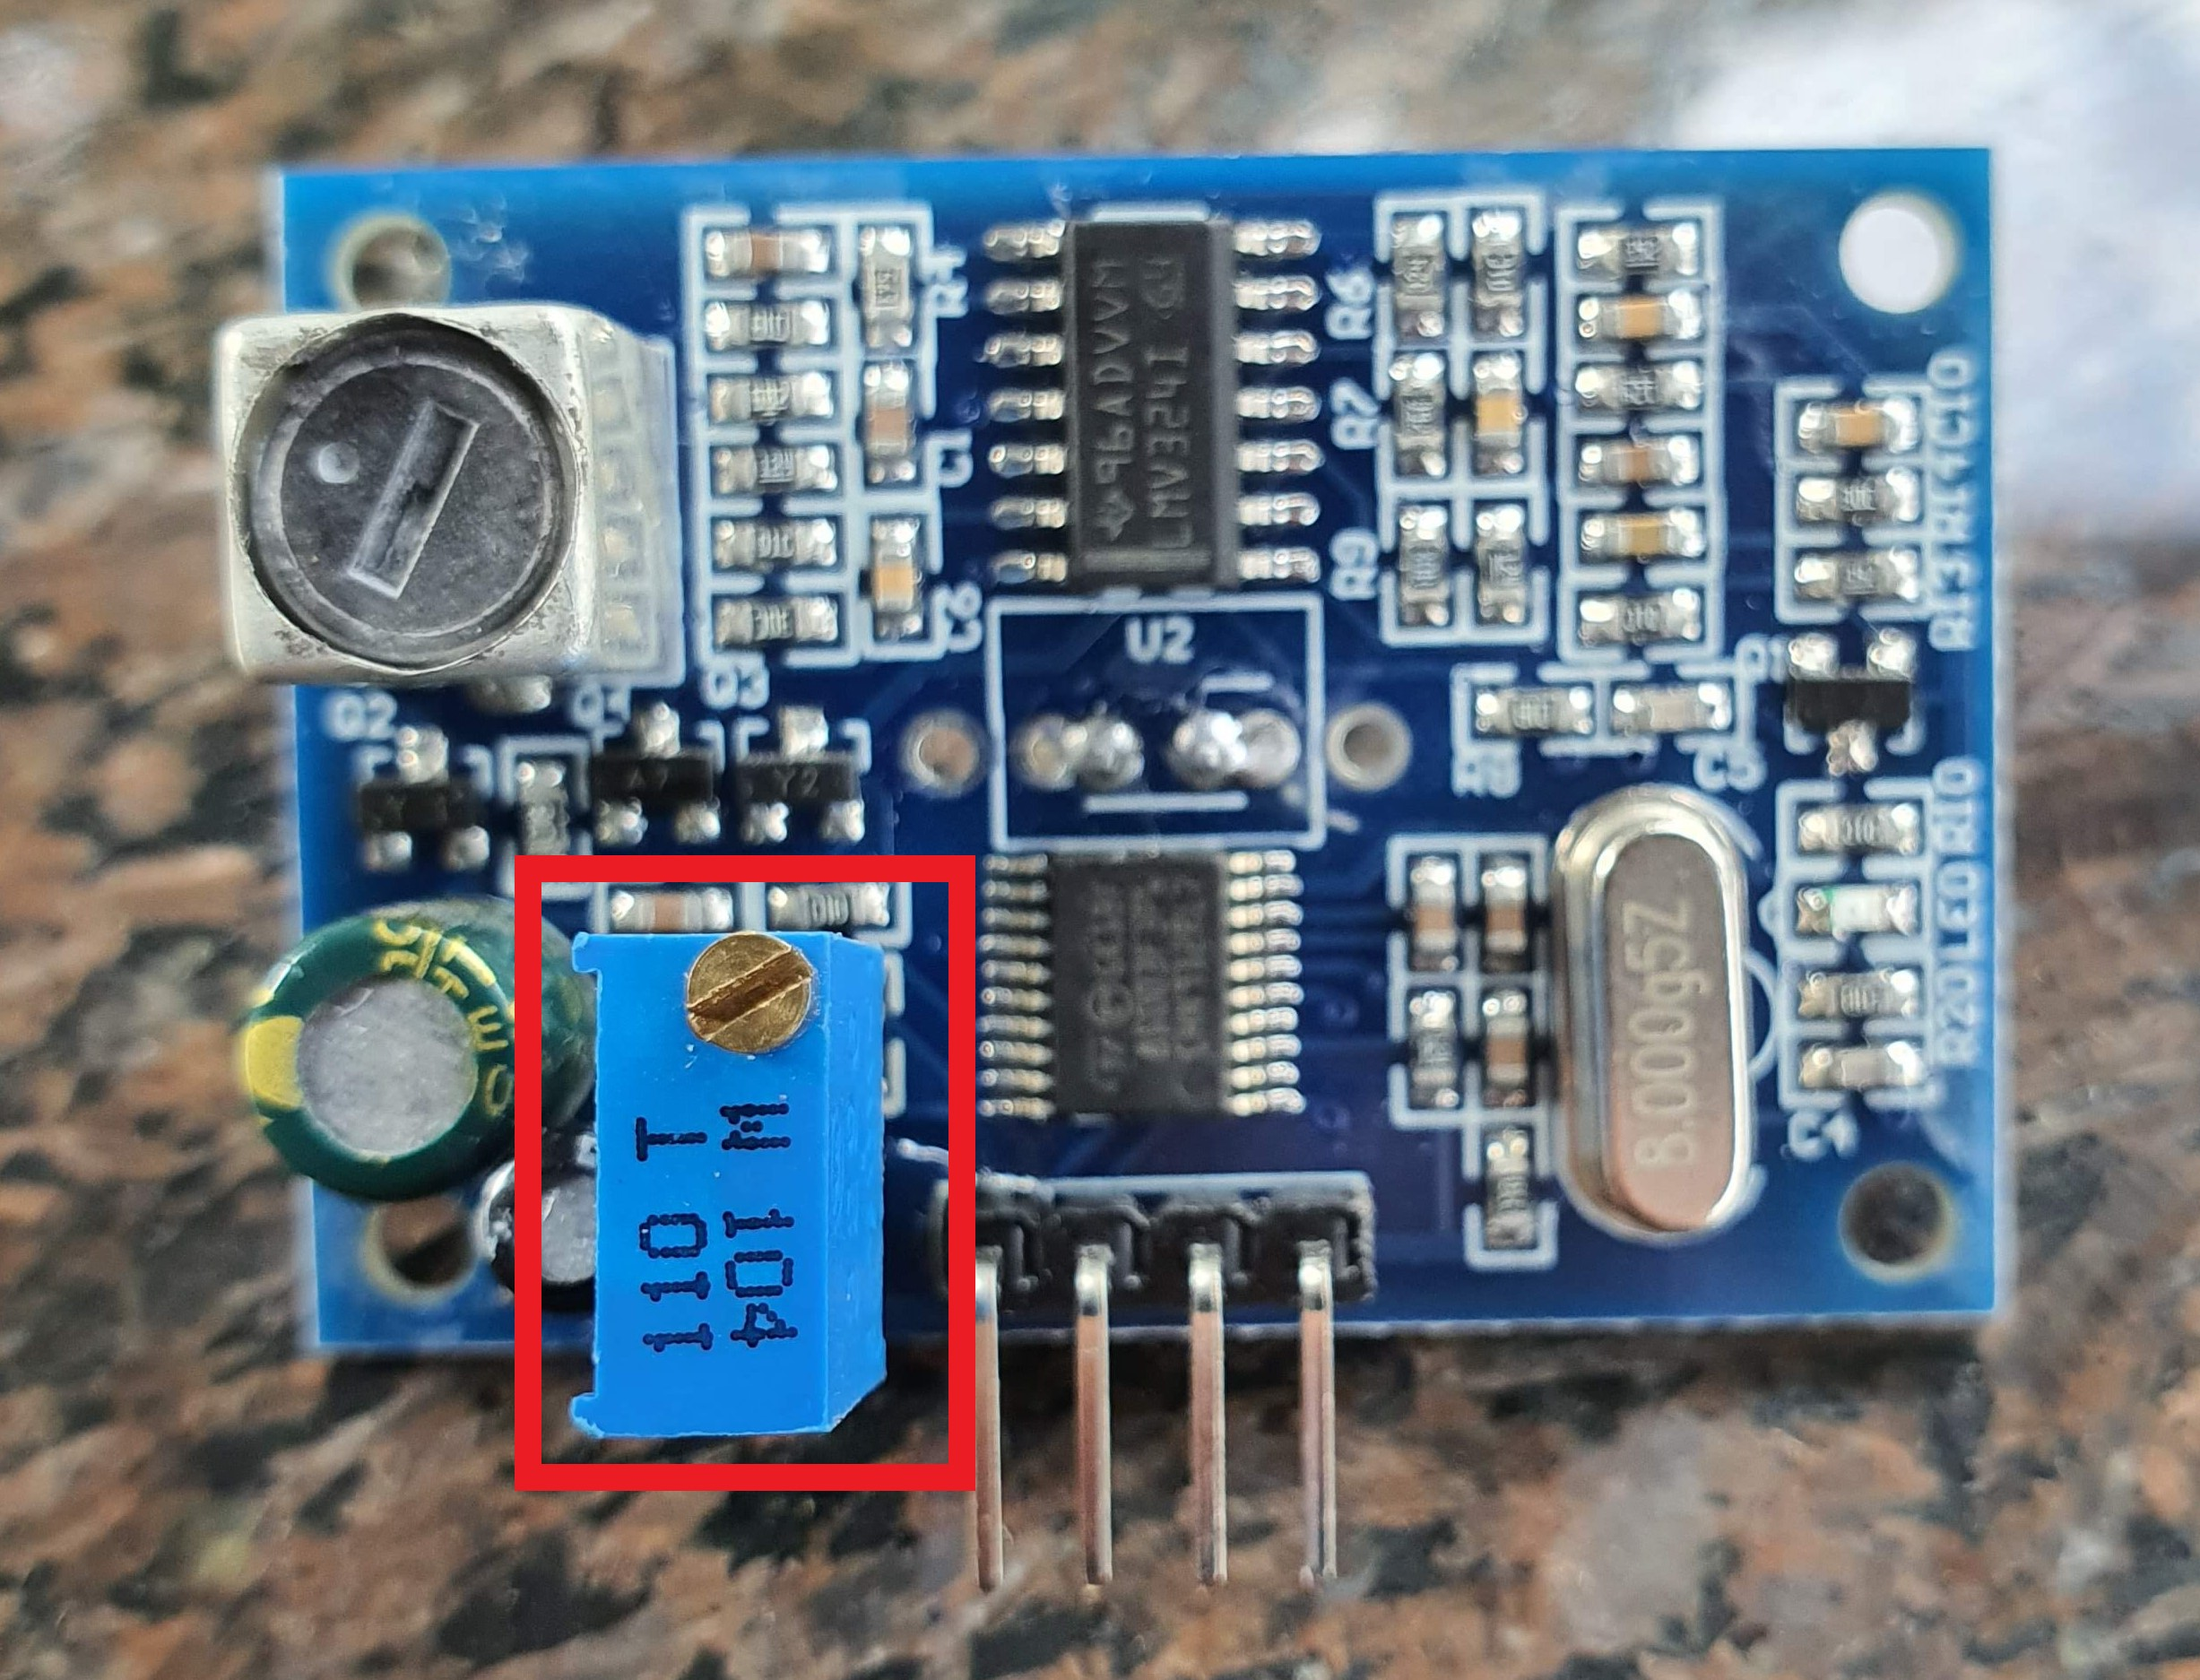
\includegraphics[width=0.6\textwidth]{figuras/ultrassonico_res.jpg}
	\fonte{Própria.}
	\label{fig:ultrasonico_res}
\end{figure}

\subsection{O circuito de ativação da motobomba}

Nesta etapa do projeto deu-se inicio a criação do controlador da motobomba. O diagrama a abaixo mostra um visão geral dos itens que precisaram ser integralizados para a ativação e desativação do motor por meio do microcontrolador.

 \begin{figure}[H]
	\centering
	\caption{Diagrama de ativação do motor}
	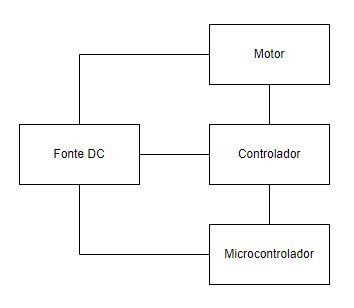
\includegraphics[width=0.4\textwidth]{figuras/ativacao_motor.png}
	\fonte{Própria.}
	\label{fig:diagrama_ativacao_motor}
\end{figure}


 Como visto, a motobomba selecionada opera com 12V em corrente contínua e, por meio de testes feitos, possui um consumo médio de 10A quando está em operação. (\autoref{fig:teste_ativacao_motor}).
 
  \begin{figure}[H]
 	\centering
 	\caption{Teste da motobomba}
 	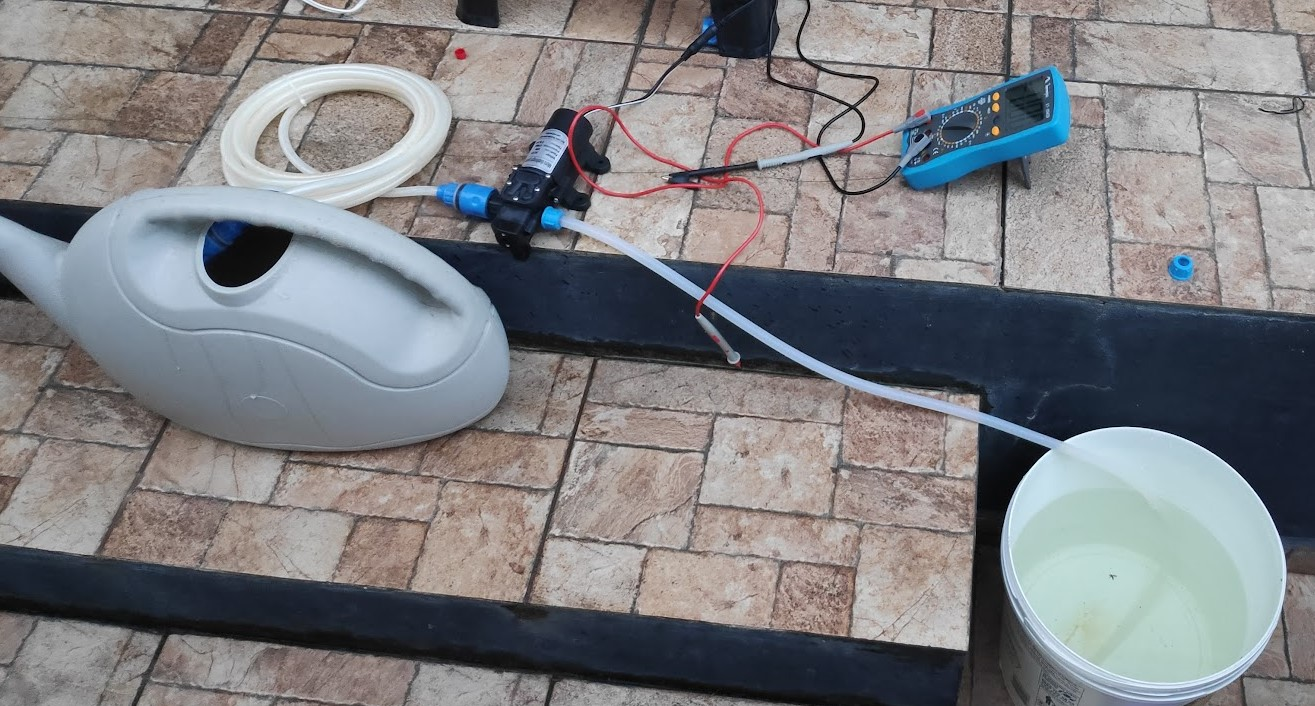
\includegraphics[width=0.6\textwidth]{figuras/teste_motor.jpg}
 	\fonte{Própria.}
 	\label{fig:teste_ativacao_motor}
 \end{figure}

Com os dados obtidos através dos testes, deu-se início a procura de componentes e metodologias para o controle \textit{ON-OFF} de motores de corrente contínua. Como o microcontrolador não possui tesão nem corrente suficientes para ativar o motor, foi-se necessário desenvolver uma ativação indireta transistorizada.  

A primeira parte do esquema (\autoref{fig:diagramaproteus} [B]) conta com o transistor MOSFET  IRF1404 de alta potência. Esse transistor, segundo seu \textit{datasheet} (recorte presente no \textbf{anexo C}), pode operar com uma corrente máxima de dreno igual a 75A e necessita de uma diferença mínima de 4V entre o $V_{GS}$ e $V_{DS}$ para conduzir a corrente $I_{DS}$.
Com essas informações chegamos a conclusão de que a tensão aplicada ao GATE deveria ser, de no mínimo, 14V.

Partindo-se disso, procurou-se técnicas para elevação de tensão e selecionamos construir um \textbf{dobrador de tensão}. Por ser simples e barato para ser desenvolvido, existem inúmeras aplicações que utilizam esse método para ativação de transistores MOSFET. Este circuito é baseado em resitores, capacitores, diodos e necessita de um oscilador conectado na base de transistor para executar ações de chaveamento. 

A \autoref{fig:dobrador_osciloscopio} mostra o comportamento da saída do dobrador montado (\autoref{fig:dobrador_montado}). Onde temos a saída de tensão (em vermelho) e a entrada de tensão 12V da fonte DC (em verde). É importante salientar que a tesão de saída atingiu valores em torno de 22V devido as perdas dos componentes, porém valor suficiente para ativar o IRF1404.
As ações de chaveamento foram feitas através de \textit{Pulse-Width Modulation - PWM} originados do ESP-12S.
\begin{figure}[H]
	\centering
	\caption{Resultados obtidos da leitura de pontos estratégicos do dobrador de tensão montado}
	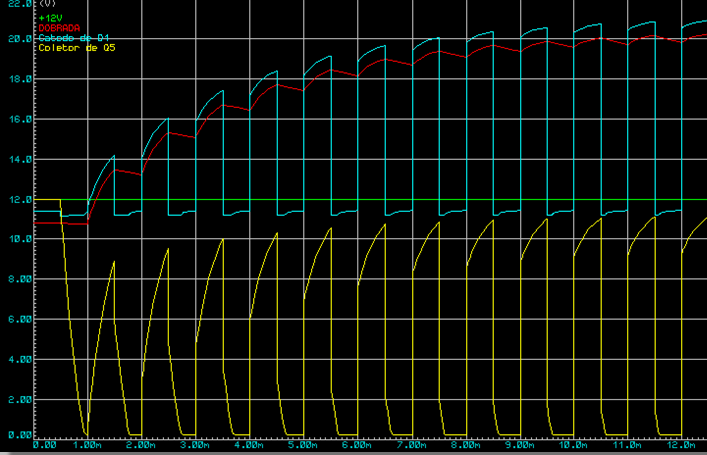
\includegraphics[width=0.8\textwidth]{figuras/dobrador.png}
	\fonte{Própria}
	\label{fig:dobrador_osciloscopio}
\end{figure}

A próxima etapa de implementação do controlador \textit{ON-OFF} foi interligar a saída do dobrador de tensão com o GATE do IRF1404. Para isso utilizamos um circuito com o transistor BC546 (\autoref{fig:diagramaproteus} [C]), o qual garante que um pino digital do microcontrolador possa ativar ou desativar a motobomba. Outra característica dessa ligação é possibilitar um \textit{soft start}\footnote{\textbf{soft start:} técnica que diminui a corrente de partida, diminuindo os choques mecânicos do motor por meio de uma aceleração constante.}, evitando picos de corrente e melhorando a vida útil do motor.

Por fim, analisando a \autoref{fig:diagramaproteus} [C] é correto afirmar que o motor será ativado quando se aplicar um nível lógico baixo no transistor Q3 e desativado ao se aplicar nível lógico alto.

\begin{figure}[H]
	\centering
	\caption{Circuito do dobrador de tensão montado.}
	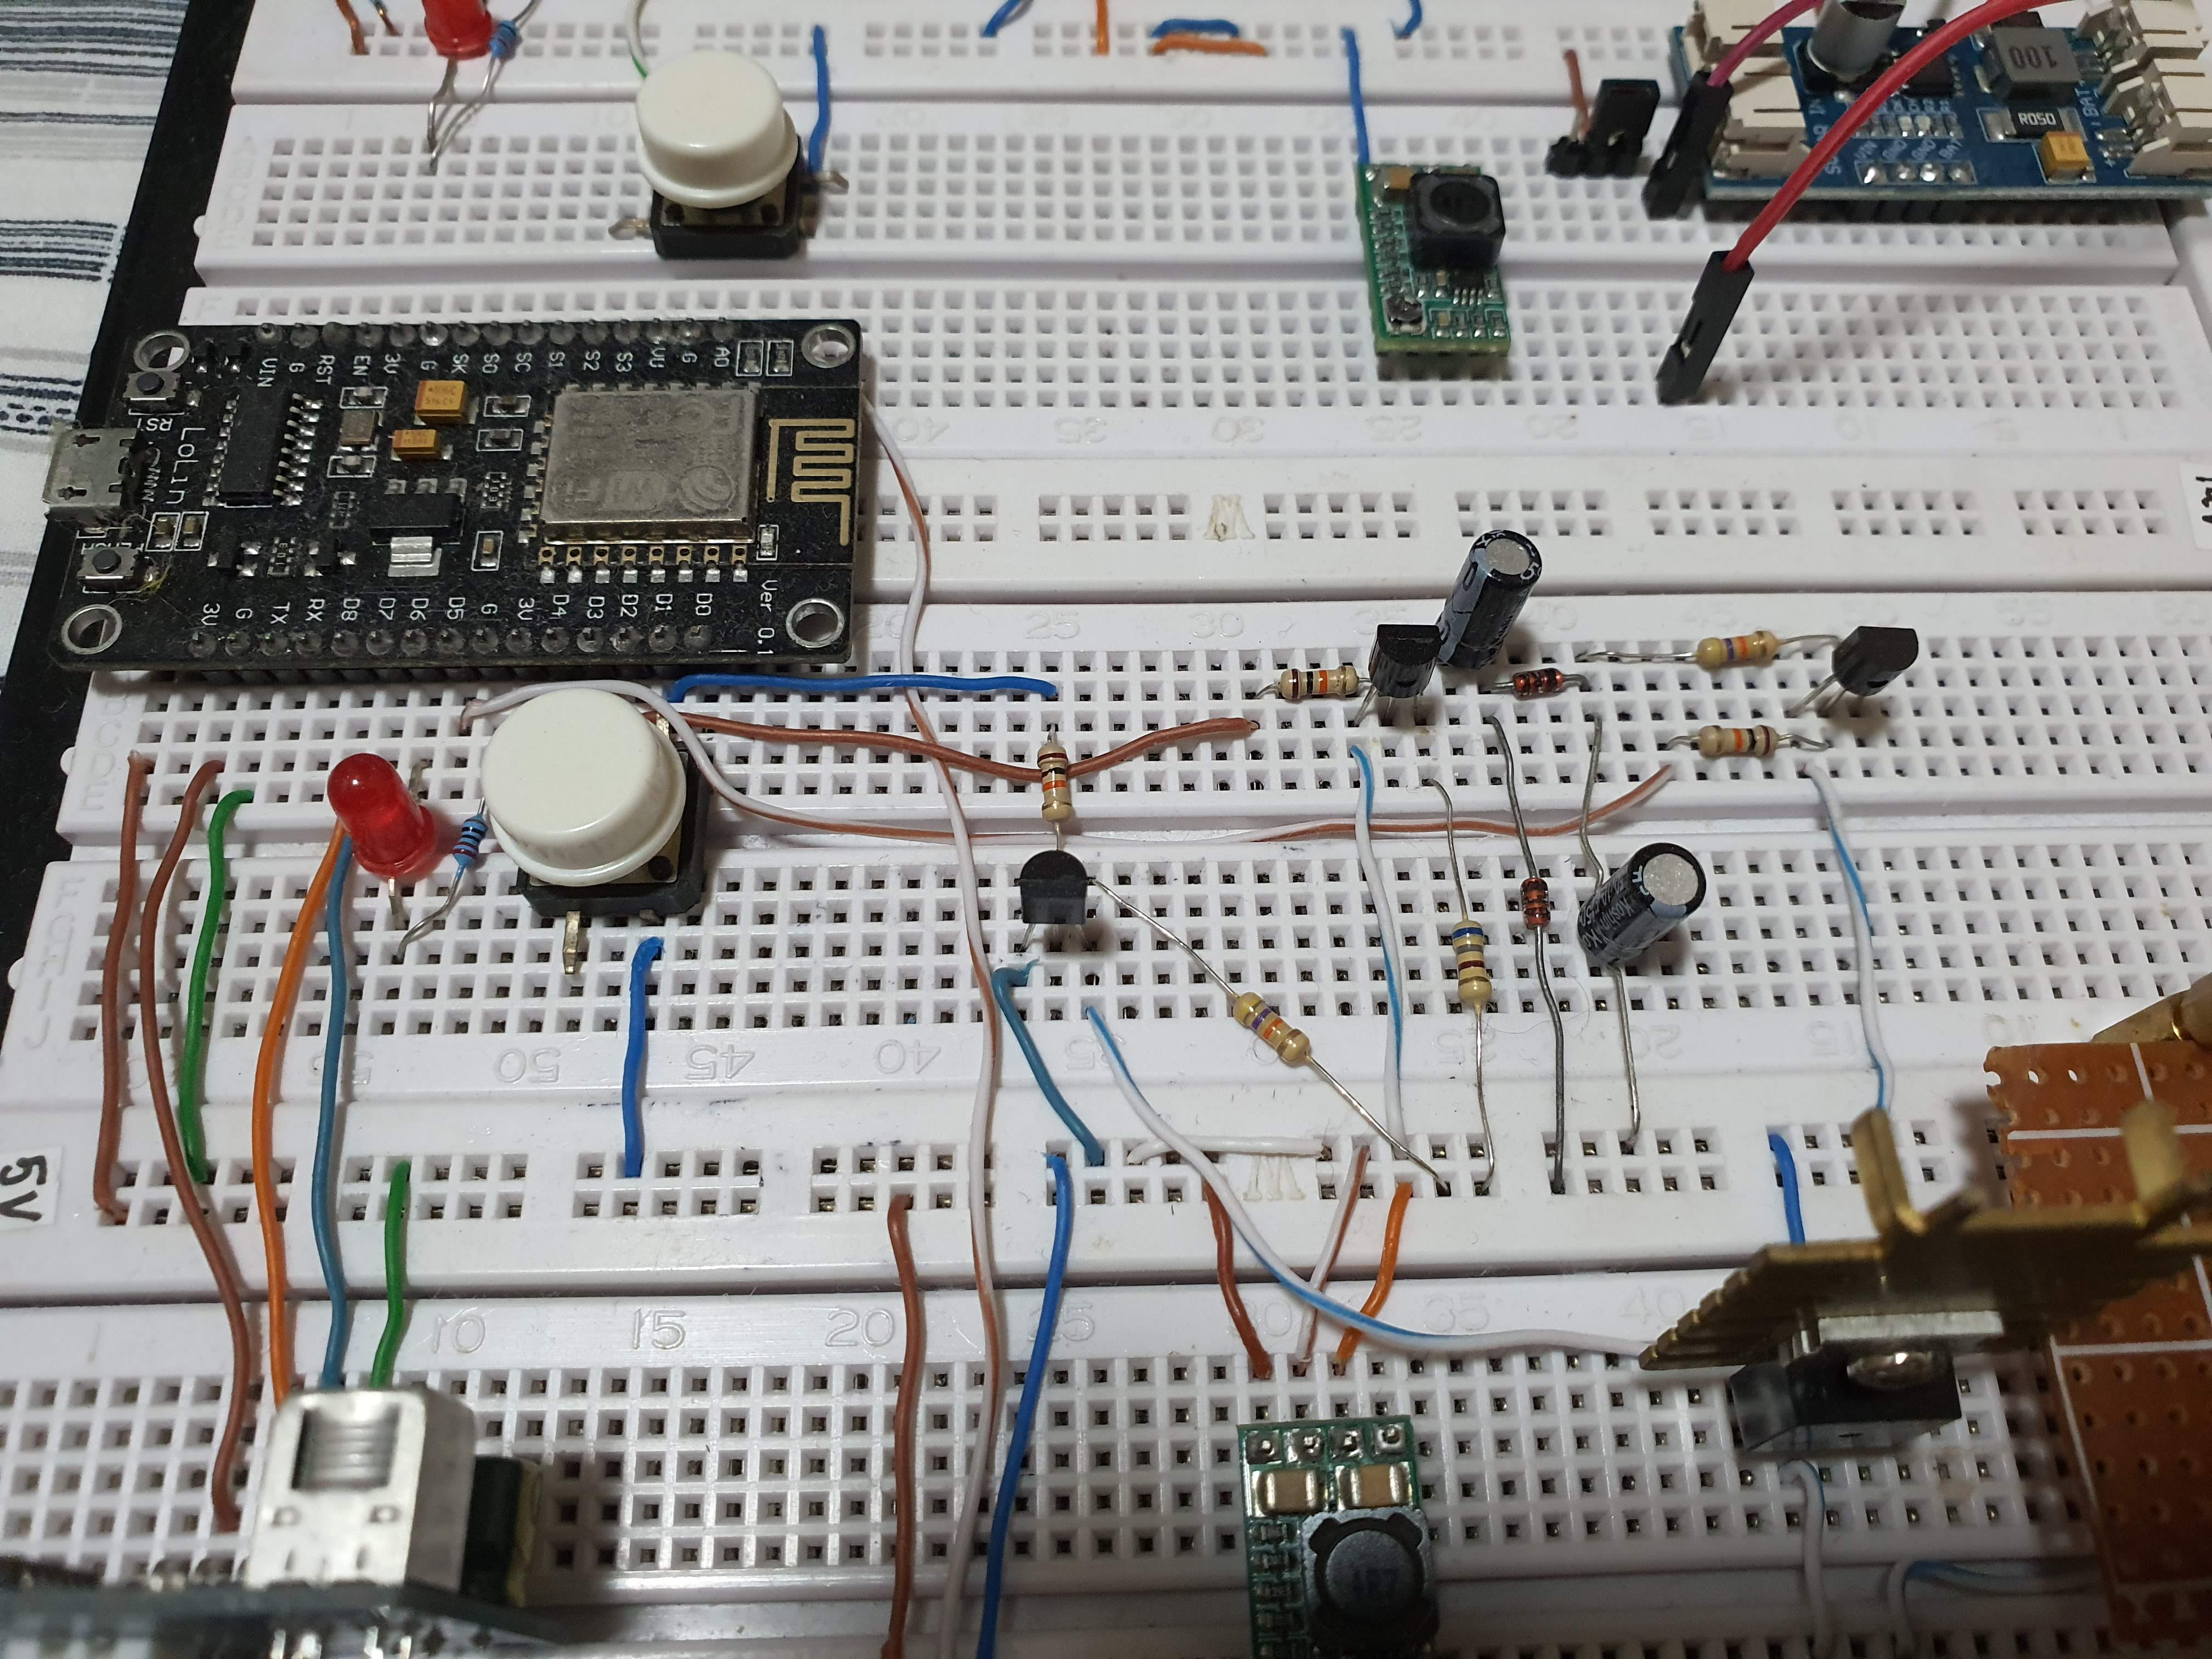
\includegraphics[width=0.6\textwidth]{figuras/dobrador_montado.jpg}
	\fonte{Própria}
	\label{fig:dobrador_montado}
\end{figure} 



\begin{figure}[H]
	\centering
	\caption{Diagrama de ativação com partida lenta}
	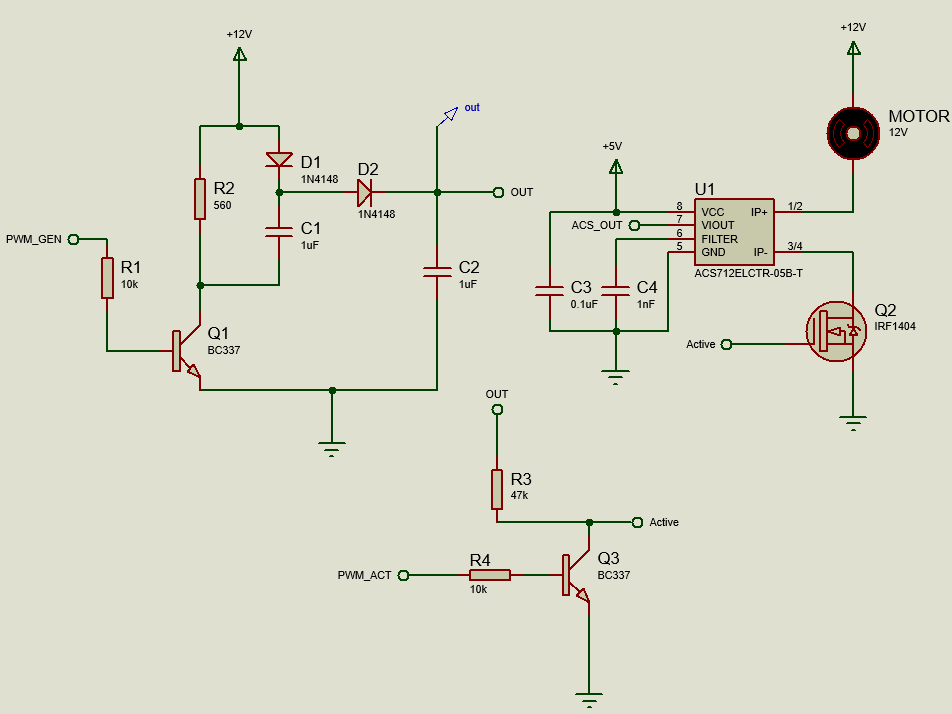
\includegraphics[width=0.9\textwidth]{figuras/diagrama_ativação_bomba.png}
	\fonte{Própria}
	\label{fig:diagramaproteus}
\end{figure} 



\subsection{O circuito de ativação da válvula}

Assim como o motobomba, a válvula solenoide da Nascimetal selecionada é ativada com tensão de 12V, necessitando também, de acordo com seu catálogo, de uma corrente em torno de $500mA$.

O circuito proposto para a ativação dessa válvula tem como dispositivo principal o transistor MOSFET IRLZ44N. Ele possui a capacidade de operar com corrente de dreno próxima ao valor de 20A, de acordo com seu \textit{datasheet}.

Para efetuar o controle da válvula a partir de um pino digital do microcontrolador, houve a necessidade de adicionar mais um circuito transistorizado, utilizando o BC546 novamente.


\begin{figure}[H]
	\centering
	\caption{Diagrama de ativação da válvula solenoide.}
	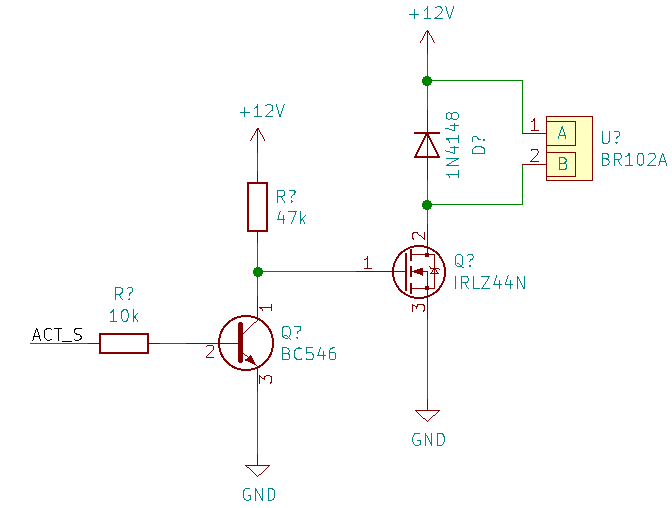
\includegraphics[width=0.6\textwidth]{figuras/ativa_valvula.png}
	\fonte{Própria}
	\label{fig:diagramavalvula}
\end{figure} 

 Novamente, observando a \autoref{fig:diagramavalvula}, percebe-se que a ativação da válvula é feita em nível lógico baixo ao aplicar no marcador ACT\_S.

\section{Desenvolvimento dos elementos de \textit{Firmware}}
\label{sec: dev_ele_fw}

A definição e desenvolvimento dos elementos de \textit{Firmware} se deu após todos os levantamentos de requisitos do trabalho. Esse momento concentrou-se na escolha de tecnologias mais fáceis de implementação (citadas na fundamentação teórica), que tivessem uma gama de documentações e que fossem empregadas em produtos oficiais. Para lidar com o uso dos microprocessadores e microcontroladores, foram feitas pesquisas visando consolidar conceitos aprendidos durante o curso de graduação.

\subsection {Instalação e configuração do \textit{Broker MQTT}}

No primeiro momento desta etapa pesquisou-se os principais serviços de \textit{broker} disponíveis, tendo em vista pontos como documentação e baixo custo. Com isso o serviço selecionado foi o Eclipse Mosquitto™.

A configuração do \textit{broker} leva em consideração quatro informações: \textbf{endereço de IP}, \textbf{porta}, \textbf{usuário} e \textbf{senha}.

Estando a Raspberry Pi Zero W rodando o sistema operacional DietPi e possuindo conexão com a \textit{internet}, a instalação do \textit{broker} e dos serviços de \textit{clients} foram realizadas através dos seguintes comandos no terminal:

\begin{lstlisting}
sudo apt-get install mosquitto
sudo apt-get install mosquitto-clients
\end{lstlisting}


Buscando garantir a segurança de acesso ao \textit{broker} realizou-se os seguintes passos no terminal a fim de configurar um usuário com senha:


\begin{lstlisting}
sudo stop mosquitto
sudo mosquitto_passwd -c /etc/mosquitto/passwd <user_name>
\end{lstlisting}

O usuário é definido em \textit{<user\_name>} e a senha foi solicitada posteriormente. Esses dados são criptografados e salvos no arquivo de configuração presente em: \textbf{/etc/mosquitto/mosquitto.conf} (\autoref{fig:cred_mqtt}).

\begin{figure}[H]
	\centering
	\caption{Arquivo de credenciais do Mosquitto gerado}
	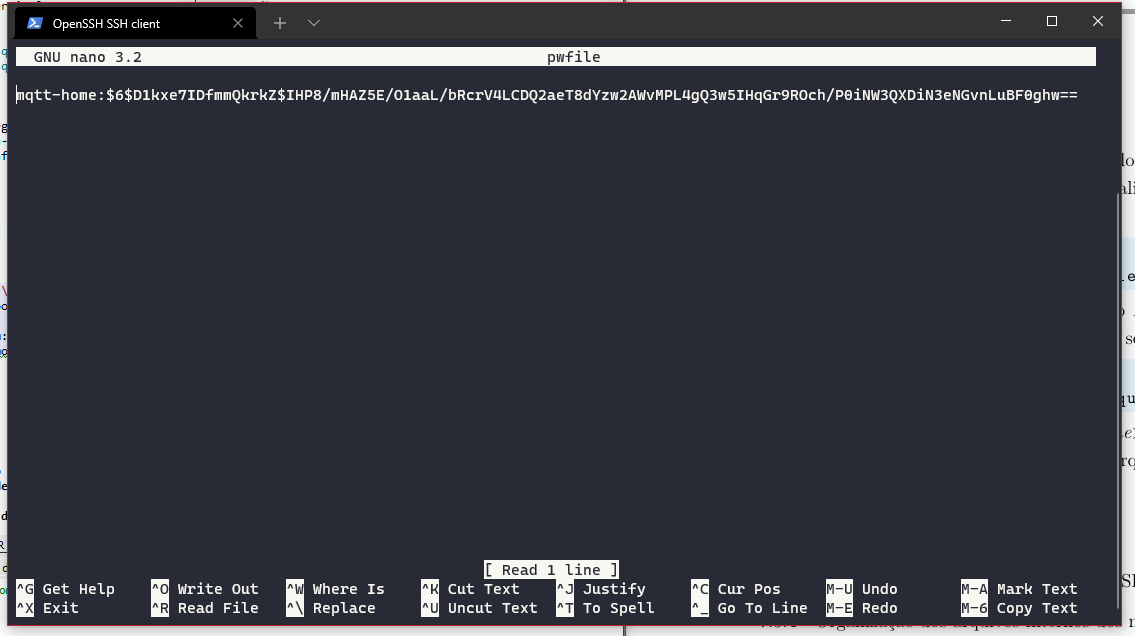
\includegraphics[width=0.6
	\textwidth]{figuras/user_pass.png}
	\fonte{Própria}
	\label{fig:cred_mqtt}
\end{figure}

Para que os clientes executem a conexão com o servidor \textit{broker} também foi necessário configurar um IP estático. Essa operação se deu acessando as configurações do roteador local (\autoref{fig:roteador}).

\begin{figure}[H]
	\centering
	\caption{Em destaque, IP estático configurado no roteador local.}
	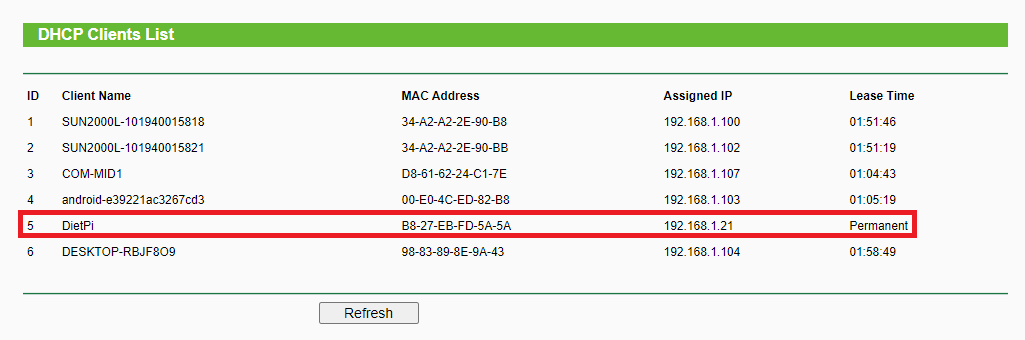
\includegraphics[width=1
	\textwidth]{figuras/ip_estatico_rasp.png}
	\fonte{Própria}
	\label{fig:roteador}
\end{figure}



\subsection {Programação do servidor}
\subsection {Definição de utilização dos pinos do ESP-12S}

Neste estágio do projeto, organizou-se a ligação de cada pino do microcontrolador esp8266, tendo em vista as características citadas no \textbf{Anexo A}. A figura abaixo mostra a organização final.

\begin{figure}[H]
	\centering
	\caption{Declarações dos pinos realizadas no código do módulo \textbf{CCM}.}
	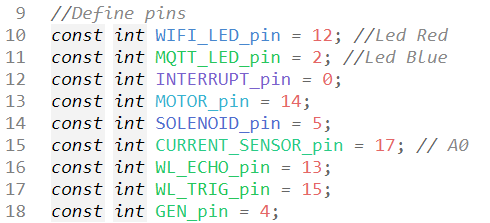
\includegraphics[width=0.5
	\textwidth]{figuras/pinos_definicao_ccm2.png}
	\fonte{Própria}
	\label{fig:definicao_pinos_ccm}
\end{figure}

\begin{figure}[H]
	\centering
	\caption{Declarações dos pinos realizadas no código do módulo \textbf{TCM}.}
	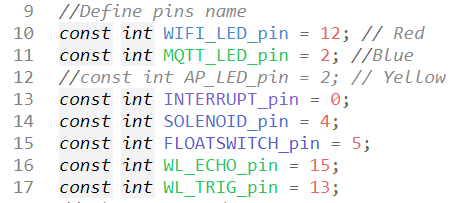
\includegraphics[width=0.5
	\textwidth]{figuras/pinos_definicao_tcm.png}
	\fonte{Própria}
	\label{fig:definicao_pinos_tcm}
\end{figure}


De acordo com as figuras, pontuamos:

\begin{itemize}
	\item \textbf{WIFI\_LED\_pin}: define o pino de conexão \textit{WI-FI};
	\item \textbf{MQTT\_LED\_pin}: define o pino de indicação de conexão MQTT;
	\item \textbf{INTERRUPT\_pin}: define o pino de interrupção para execução de \textit{Reset};
	\item \textbf{MOTOR\_pin}: define o pino de ativação e desativação da motobomba;
	\item \textbf{GATE\_pin}: define o pino de ativação e desativação da válvula solenoide;
	\item \textbf{FLOATSWITCH\_pin}: define o pino da chave do tipo boia;
	\item \textbf{CURRENT\_sensor\_pin}: define o pino de leitura do sensor de corrente (pino analógico);
	\item \textbf{WL\_ECHO\_pin}: define um pino de comunicação com o módulo ultrasônico JSN-SR04T;
	\item \textbf{WL\_TRIG\_pin}: define um pino de comunicação com o módulo ultrasônico JSN-SR04T; 
\end{itemize}


\subsection{Organização dos arquivos internos dos microcontroladores}

Utilizando uma biblioteca chamada \textit{SPIFFS}, nesta etapa do desenvolvimento do \textit{firmware} dos módulos, foi implementado um sistema de arquivos na memória \textit{flash} dos microcontroladores ESP-12S. 

Esse sistema de arquivos, gravados na memória não-volátil, tem como objetivo armazenar dados pertinentes como: a versão do \textit{firmware}, os dados para conexão WI-FI e MQTT, além de armazenar páginas \textit{HTML} para o processo de cadastro, o qual será descrito no quesito 7.5.6.

% Please add the following required packages to your document preamble:
% \usepackage{graphicx}
\begin{table}[H]
	\centering
	\resizebox{\textwidth}{!}{%
		\begin{tabular}{c|c}
			\hline
			Arquivo &  Função \\ \hline
			system\_info.json &  \begin{tabular}[c]{@{}c@{}} armazena a versão do firmware, versão do sistema de arquivos,\\ data do ultimo update e o link para o repositório de novos binários \end{tabular} \\ \hline
			register\_config.json &  \begin{tabular}[c]{@{}c@{}} armazena os dados para conexão WI-FI (\textit{ssid} e senha) e os dados para conexão ao \\ \textit{broker} MQTT (IP, porta, usuário, senha, tópico de inscrição e o tópico de publicação) \end{tabular} \\ \hline
			new\_network.html & \begin{tabular}[c]{@{}c@{}} página para cadastro de do dispositivo na rede WI-FI e ao servidor MQTT \end{tabular} \\ \hline
			confirm.html & \begin{tabular}[c]{@{}c@{}} página de confirmação para recebimento dos dados após o cadastro \end{tabular}  \\ \hline
		\end{tabular}%
	}
	\caption{Descrição dos arquivos salvos na memória interna do microcontrolador.}
	\label{tab:file_system_esp}
\end{table}

\subsection{Comunicação com o sensor de nível}

Como visto anteriormente módulo JSN-SR04T possui três modos de operação. Para este trabalho selecionou-se o modo \textbf{3} por utilizar o controlador da placa e por permitir um baixo consumo. A função evidenciada na \autoref{fig:code_jsn-sr04t} é chamada sempre que se deseja realizar uma leitura de distância. Ela envia o comando 0x55 via serial e aguarda a resposta do módulo. Quando a resposta chega, ela é segmentada e armazenada na variáveis: \textit{startByte}, \textit{h\_data}, \textit{l\_data} e \textit{sum}. A validação é feita através da comparação: 
\begin{lstlisting}
if ((startByte + h_data + l_data) != sum)
\end{lstlisting}

Se o valor a comparação for igual a função retorna o valor lido em milímetros, se não for retorna o valor zero.


\begin{figure}[H]
	\centering
	\caption{Função para realizar a leitura de distância a partir do sensor ultrassônico.}
	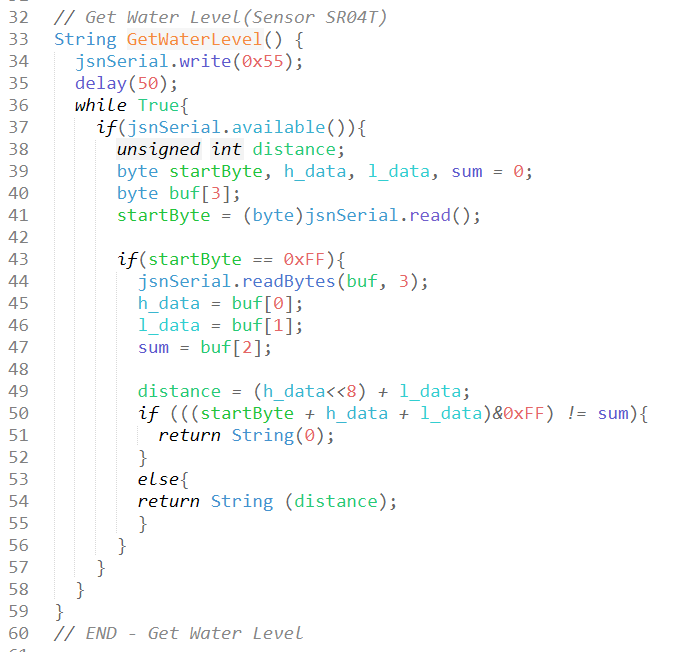
\includegraphics[width=0.7
	\textwidth]{figuras/get_water_level.png}
	\fonte{Própria}
	\label{fig:code_jsn-sr04t}
\end{figure}



\subsection {Implementação do \textit{Driver WI-FI}}

Esta seção concentra-se em explicar o conjunto de funções criadas, organizadas no arquivo de cabeçalho \textit{Driver\_WIFI.h}, as quais lidam com as rotinas de conexão e desconexão assim como as operações de cadastro do dispositivo. Um módulo, seja ele um \textbf{TCM} ou \textbf{CCM}, na sua primeira utilização será necessário configurar: a rede \textit{WI-FI} para se conectar, o servidor \textit{broker} e os tópicos de inscrição e de publicação. Esse cadastro é realizado a partir de uma página \textit{HTML} (\autoref{fig:cadastro}) gerada pelo microcontrolador, que nos estágios iniciais se comporta como um ponto de acesso (\textit{Access Point)}. É importante notar que se o módulo perder conexão com o \textit{WI-FI} ou com o servidor \textit{MQTT} ele irá entrar no modo de alternância: 3 minutos tentando uma reconexão e 5 minutos com um ponto de acesso disponível para uma nova configuração.

 O diagrama da \autoref{fig:firmware_sequence} mostra o comportamento completo do \textit{firmware} após o \textit{boot} \footnote{\textbf{\textit{boot}}: termo utilizado para fazer referência ao processo de inicialização de um dispositivo microcontrolado ou microprocessado.} do microcontrolador.

\begin{figure}[H]
	\centering
	\caption{Diagrama de operação do microcontrolador.}
	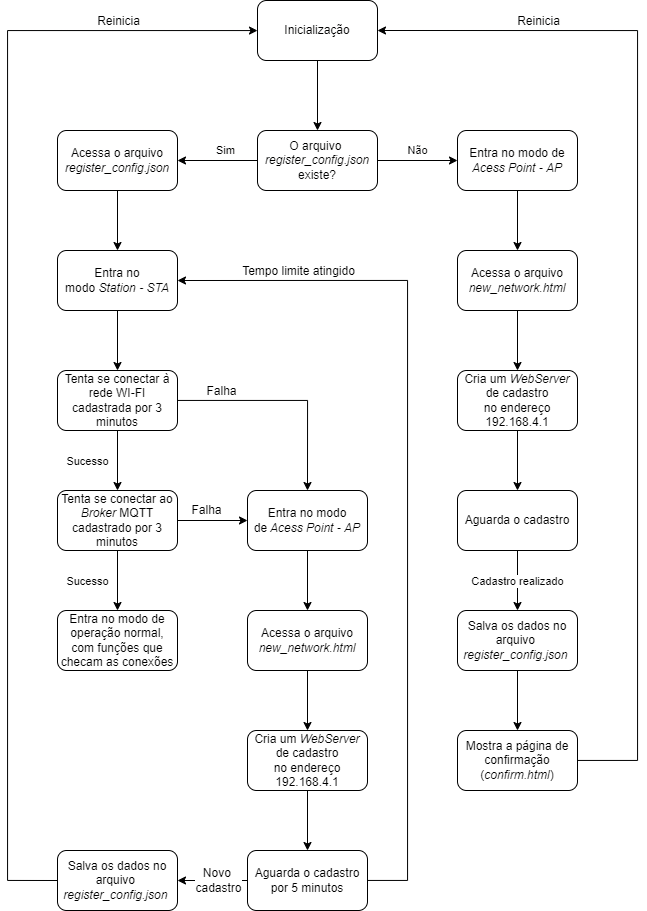
\includegraphics[width=1\textwidth]{figuras/firmware_sequence.png}
	\fonte{Própria}
	\label{fig:firmware_sequence}
\end{figure}

\begin{figure}[H]
	\centering
	\caption{Página \textit{HTML} gerada para cadastro do dispositivo.}
	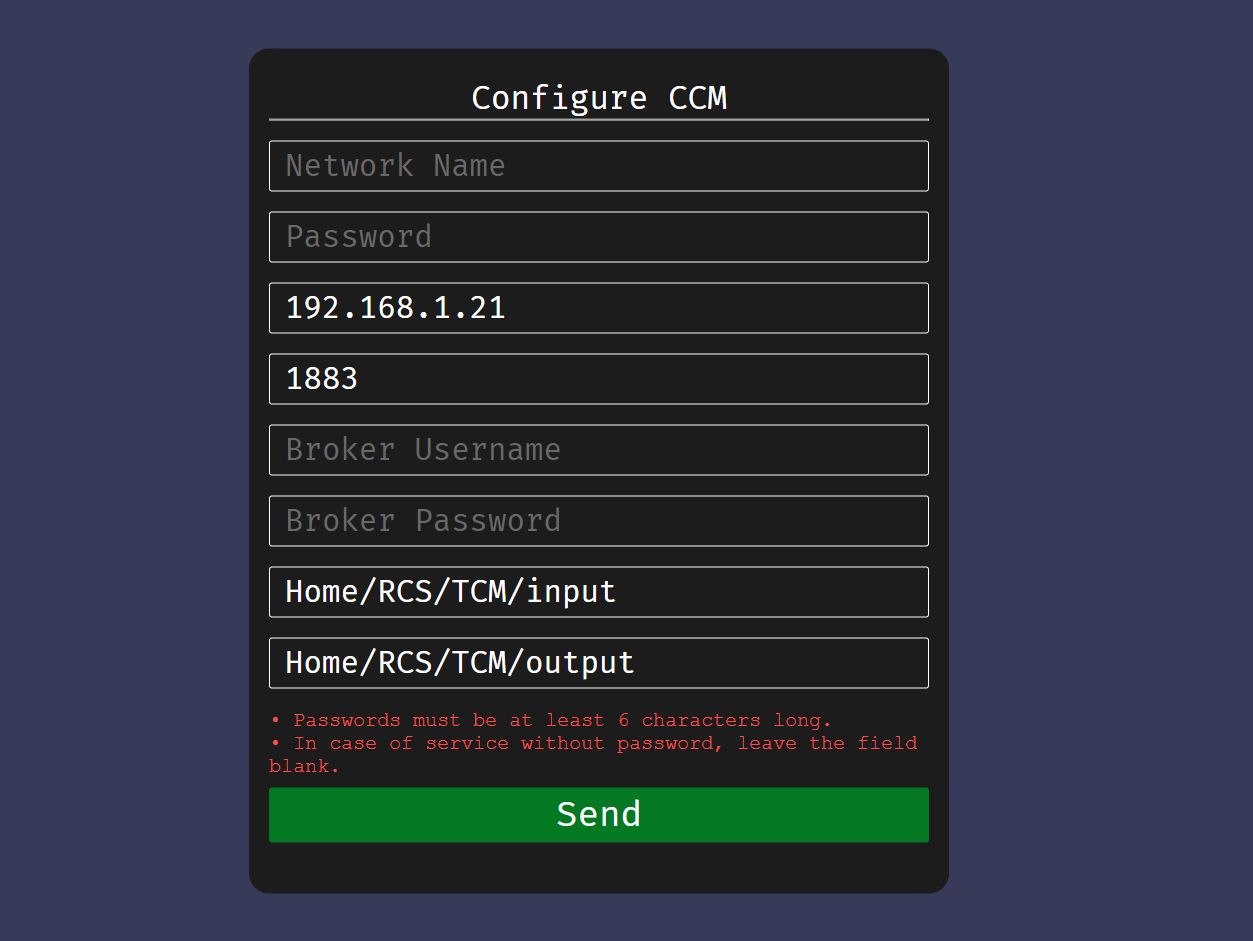
\includegraphics[width=0.8\textwidth]{figuras/cadastro_client.png}
	\fonte{Própria}
	\label{fig:cadastro}
\end{figure}

\subsection {Implementação do \textit{Driver MQTT}}

Estando um módulo devidamente cadastrado, em modo normal de operação, ele utiliza as funções de \textit{MQTT}. A biblioteca que permite as ações de conexão, publicação e inscrição com o procolo \textit{MQTT} se chama \textit{PubSubClient}. Com a utilização desse biblioteca foi-se possível configurar o \textit{\textbf{QoS}} = 2, assegurando uma troca de mensagens de forma mais confiável.

Nesta etapa da produção de código, foi criado um \textit{callback} o qual executa ações de acordo as mensagens que chegam no tópico em o \textit{client} \textbf{TCM} ou \textbf{CMM} está inscrito. Esse callback pode é apresentado na \autoref{fig:drive_mqtt}.

\begin{figure}[H]
	\centering
	\caption{Função de \textit{Callback}.}
	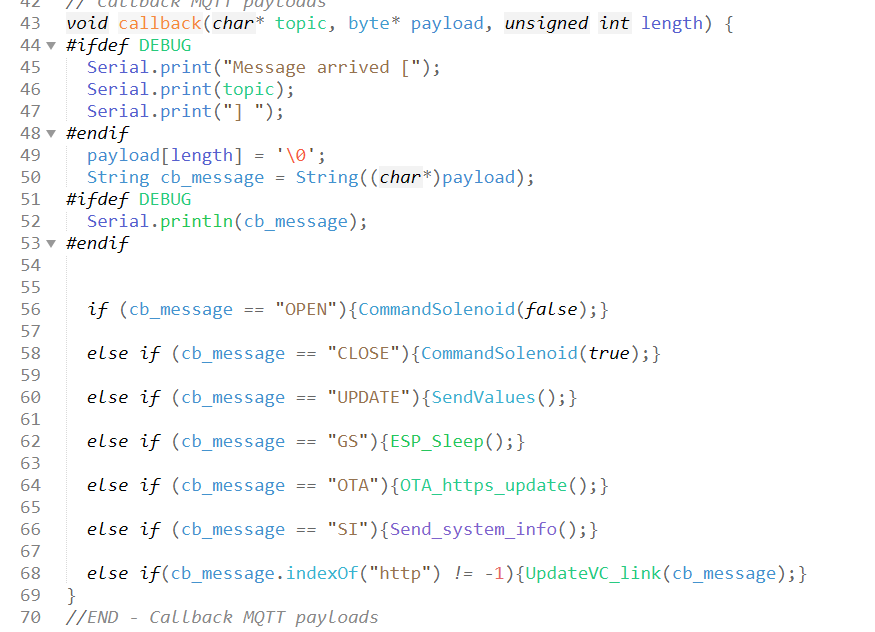
\includegraphics[width=0.8\textwidth]{figuras/drive_mqtt.png}
	\fonte{Própria}
	\label{fig:drive_mqtt}
\end{figure}

Ao receber uma mensagem no tópico em que está inscrito, o programa valida a mensagem que deve ser e executa as ações de acordo com as condições.

% Please add the following required packages to your document preamble:
% \usepackage{graphicx}
% Please add the following required packages to your document preamble:
% \usepackage{graphicx}
\begin{table}[H]
	\centering
	\resizebox{12cm}{!}{
		\begin{tabular}{c|c}
			\hline
			Mesagem     & Ação                                                  \\ \hline
			ON          & Liga a motobomba                                      \\ \hline
			OFF         & Desliga a motobomba                                   \\ \hline
			OPEN        & Abre a válvula solenoide                              \\ \hline
			CLOSE       & Fecha a válvula solenoide                             \\ \hline
			UPDADE      & Retorna um arquivo json com os dados sesores          \\ \hline
			GS          & Coloca o processador em modo de DeepSleep             \\ \hline
			OTA         & Verifica se há uma atualização de firmware disponível \\ \hline
			SI          & Retorna o um arquivo json com os dados do sistema     \\ \hline
			HTTP + LINK & Cadastra um novo link para busca de atualizações      \\ \hline
		\end{tabular}%
	}
	\caption{Comandos válidos para os módulos TCM e CCM}
	\label{tab:mqtt_commands}
\end{table}


\subsection{Implementação do \textit{Factory Reset}}

Como visto nas seções anteriores, as ações do microcontrolador são tomadas a partir do arquivo de configuração \textit{register\_config.json}. A rotina de \textit{Factory Reset} \footnote{\textbf{Factory Reset}: procedimento que faz um determinado dispositivo eletrônico retornar ao seu estado original de fábrica.} implementada tem como objetivo levar o microcontrolador ao estado inicial presente na figura. Para que isso aconteça é necessário apenas apagar o arquivo \textit{register\_config.json} e reiniciar dispositivo.

Tomou-se como base as implementações de \textit{Factory Reset} de roteadores, as quais são executadas a partir de um botão físico. O código abaixo mostra como ocorre a operação de restauração, utilizando um botão interligado à um pino de interrupção.

\begin{figure}[H]
	\centering
	\caption{Função de interrupção.}
	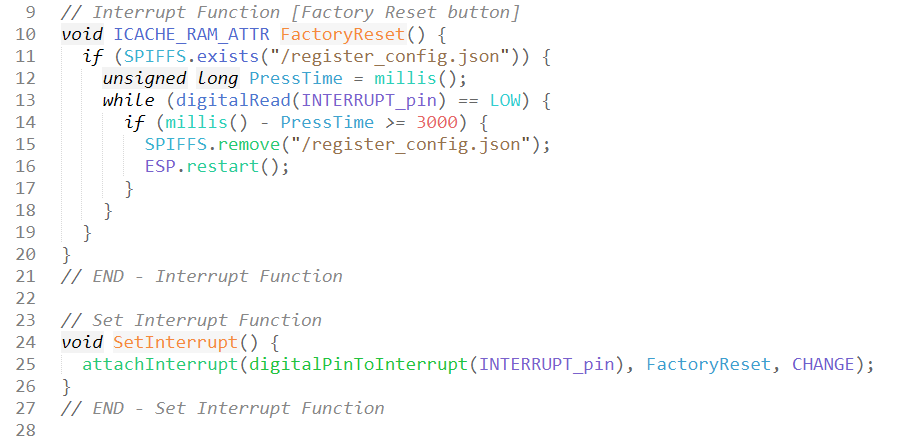
\includegraphics[width=0.8\textwidth]{figuras/interrupcao.png}
	\fonte{Própria}
	\label{fig:interrupcao}
\end{figure}


Uma interrupção é um sinal enviado por um dispositivo de \textit{hardware} (compreendido internamente no \textit{chip} do microcontrolador) que temporariamente interrompe a tarefa que a \textit{CPU} está executando no momento, para executar uma ação pré-estabelecida. Logo após, o programa retoma seu processamento do ponto onde havia parado. No caso de interrupções externas, o esp8266 aceita 5 modos distintos:

\begin{itemize}
	\item CHANGE – Interrupção é disparada quando o pino muda de estado;
	\item FALLING – Interrupção é disparada quando o pino vai do estado HIGH para LOW;
	\item HIGH – Interrupção é disparada quando o pino está no nível HIGH;
	\item LOW – Interrupção é disparada quando o pino está no nível LOW;
	\item RISING – Interrupção é disparada quando o pino vai do estado LOW para HIGH.
\end{itemize}

Na \autoref{fig:interrupcao} a função \textit{SetInterrupt()} define qual função deve ser executada durante a interrupção e qual o modo de disparo. A função \textit{ICACHE\_RAM\_ATTR FactoreReset()} remove o arquivo \textit{register\_config.json} e reinicia o microcontrolador se o botão for pressionado por mais de 3 segundos.



\subsection{Implementação da funcionalidade de \textit{OTA Upgrade}}


\section{Desenvolvimento dos elementos de \textit{Software}}


Para o desenvolvimento dos elementos de \textit{Software} buscou-se a participação de cursos básicos e avançados sobre aplicações \textit{front-end}, as quais servem de conteúdo complementar aos temas abordados na graduação em engenharia de controle e automação.

Os cursos adquiridos trouxeram uma série de conhecimentos para uma maior interação entre desenvolvedor e usuário, possibilitando a criação de interfaces intuitivas e agregando novas informações e visões a outros temas, como na programação de sistemas embarcados.




\section{Desenvolvimento da aplicações \textit{Desktop} e \textit{Mobile}}

O desenvolvimento das aplicações \textit{desktop} e \textit{mobile} tiveram início com a formulação da tela utilizando o \textit{Figma}. Primeiramente selecionamos a paleta de cores para garantir um \textit{software} mais atraente visualmente e a partir disso alguns esboços foram criados. Uma das preocupações, foi garantir que os mostradores e botões fossem bem compreendidos e de fácil acesso, com isso, as telas (\autoref{fig:figma_plan_desktop}) apresentaram-se convenientes.

\begin{figure}[H]
	\centering
	\caption{Definição do \textit{layout} das telas criado no Figma.}
	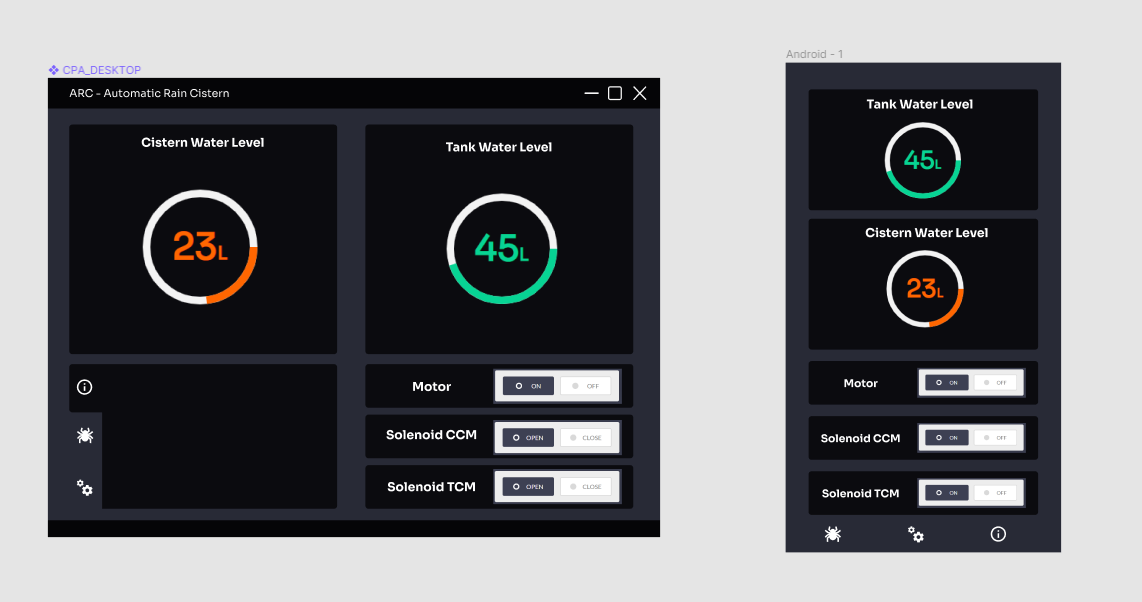
\includegraphics[width=0.6\textwidth]{figuras/figma_plan.png}
	\fonte{Própria}
	\label{fig:figma_plan_desktop}
\end{figure}



As aplicações rodam em uma única tela com quatro seções, em formato de \textit{dashboard} \footnote{\textbf{dashboard}: painel de informação e/ou controle de determinado processo.}. Nas seções superiores mostra os valores de volume da cisterna e da caixa d'água auxiliar em litros. Nas seções inferiores encontram-se os botões para ativação e desativação da motobomba, abertura e fechamento do solenoide A (presente no módulo \textbf{CCM}) e abertura e fechamento do solenoide B (presente no módulo \textbf{TCM})

Com o \textit{layout's} definidos iniciou-se o processo de criação das aplicações \textit{desktop} e \textit{mobile} como base as tecnologias \textit{Electron}, \textit{React} e \textit{React Native}.